\documentclass[preprint,5p,twocolumn,11pt,sort&compress]{elsarticle}

\usepackage{amssymb}
\usepackage{amsthm}
\setlength{\mathindent}{0pt}
\usepackage{tabularx}
\usepackage{graphicx}
\usepackage{epsfig}
\usepackage{textcomp}
\usepackage{subfigure}
\usepackage{natbib}
\usepackage[colorlinks,linkcolor=red,anchorcolor=yellow,citecolor=yellow]{hyperref}
\usepackage{color,soul}
\usepackage{multirow}
\usepackage{overpic}
\usepackage{amsmath}
\usepackage{caption}
\usepackage{bm}
\usepackage{framed}
\usepackage{threeparttable}
\usepackage{booktabs}
% \usepackage{ctex}

\newcommand{\bfsigma}{{\mbox{\boldmath{$\sigma$}}}}
\newcommand{\bfepsilon}{{\mbox{\boldmath{$\varepsilon$}}}}
\newcommand{\dotbfepsilon}{{\mbox{\boldmath{$\dot\varepsilon$}}}}
\newcommand{\dotbfsigma}{{\mbox{\boldmath{$\dot\sigma$}}}}
\newcommand{\bftau}{{\mbox{\boldmath{$\tau$}}}}
\newcommand{\bfpsi}{{\mbox{\boldmath{$\psi$}}}}
\newcommand{\bfphi}{{\mbox{\boldmath{$\phi$}}}}
\newcommand{\bfalpha}{{\mbox{\boldmath{$\alpha$}}}}
\newcommand{\bfbeta}{{\mbox{\boldmath{$\beta$}}}}
\newcommand{\bfK}{{\bf K}}
\newcommand{\bff}{{\bf f}}
\newcommand{\bfn}{{\bf n}}
\newcommand{\bfm}{{\bf m}}
\newcommand{\bft}{{\bf t}}
\newcommand{\bfu}{{\bf u}}
\newcommand{\bfw}{{\bf w}}
\newcommand{\bfa}{{\bf a}}
\newcommand{\bfb}{{\bf b}}
\newcommand{\bfs}{{\bf s}}
\newcommand{\bfB}{{\bf B}}
\newcommand{\bfD}{{\bf D}}
\newcommand{\bfnabla}{{\mbox{\boldmath{$\nabla$}}}}
\newcommand{\bfDelta}{{\mbox{\boldmath{$\Delta$}}}}
\newcommand{\bfkappa}{{\mbox{\boldmath{$\kappa$}}}}
\newcommand{\bfN}{{\bf N}}
\newcommand{\bfT}{{\bf T}}
\newcommand{\bfG}{{\bf G}}
\newcommand{\bfH}{{\bf H}}
\newcommand{\dd}{{\rm d}}
\newcommand{\marked}[1]{\textcolor{red}{#1}}

%\bibliographystyle{elsarticle-num}

% \graphicspath{{F:/Cloud/GitHub/doctor/figs/}{F:/Cloud/GitHub/doctor/figs/origin/}{F:/Cloud/GitHub/doctor/figs/tracepro/}{F:/Cloud/GitHub/doctor/figs/independent/}{F:/Cloud/GitHub/doctor/figs/python/}{F:/Cloud/GitHub/doctor/figs/ppt/}{F:/Cloud/GitHub/doctor/figs/svg/}{F:/Cloud/GitHub/doctor/figs/sem/}{F:/Cloud/Database/IN718/SEM/}{F:/Cloud/GitHub/fatigue/figs/}}

% \graphicspath{{F:/Cloud/GitHub/doctor/figs/}{F:/Cloud/GitHub/doctor/figs/origin/}{F:/Cloud/GitHub/doctor/figs/tracepro/}{F:/Cloud/GitHub/doctor/figs/independent/}{F:/Cloud/GitHub/doctor/figs/python/}{F:/Cloud/GitHub/doctor/figs/ppt/}{F:/Cloud/GitHub/doctor/figs/svg/}{F:/Cloud/GitHub/doctor/figs/sem/}{F:/Cloud/GitHub/doctor/figs/test/}{F:/Cloud/Database/IN718/SEM/}{F:/Cloud/GitHub/fatigue/figs/}{F:/Cloud/GitHub/furnace/figs/}{F:/Cloud/GitHub/tmf/figs/}{F:/Cloud/GitHub/tgmf/figs/}}

\graphicspath{{figures/}}

\journal{International Journal of Fatigue}

\begin{document}

\captionsetup[figure]{labelfont={bf},font={footnotesize},name={Fig.},labelsep=period}

\captionsetup[table]{labelfont={bf},font={footnotesize},name={Table},labelsep=period}

\renewcommand\figureautorefname{Fig.}

\sethlcolor{yellow}

\begin{frontmatter}

%% Title, authors and addresses

%% use the tnoteref command within \title for footnotes;
%% use the tnotetext command for theassociated footnote;
%% use the fnref command within \author or \address for footnotes;
%% use the fntext command for theassociated footnote;
%% use the corref command within \author for corresponding author footnotes;
%% use the cortext command for theassociated footnote;
%% use the ead command for the email address,
%% and the form \ead[url] for the home page:
%% \title{Title\tnoteref{label1}}
%% \tnotetext[label1]{}
%% \author{Name\corref{cor1}\fnref{label2}}
%% \ead{email address}
%% \ead[url]{home page}
%% \fntext[label2]{}
%% \cortext[cor1]{}
%% \address{Address\fnref{label3}}
%% \fntext[label3]{}

\title{Life assessment of thermal gradient mechanical fatigue of a nickel-based superalloy Inconel 718}

%% use optional labels to link authors explicitly to addresses:
%% \author[label1,label2]{}
%% \address[label1]{}
%% \address[label2]{}

\author{Jingyu SUN\fnref{label1}}
\author{Huang YUAN\corref{cor1}\fnref{label1}}

\address[label1]{School of Aerospace Engineering, Tsinghua University, Beijing, China\fnref{label1}}
\address[label2]{Department of Civil Engineering, Technical University of Darmstadt, Germany\fnref{label2}}
\cortext[cor1]{Corresponding author.}
\ead{yuan.huang@tsinghua.edu.cn}

\begin{abstract}
Gas turbine blades and discs are subjected to thermomechanical fatigue loadings as well as the temperature gradient induced by the internal cooling during operation. Therefore, it is necessary to evaluate the lifetime under the thermal gradient mechanical fatigue (TGMF) loading conditions.
In this study, a radiation furnace was developed for the TGMF tests. The temperature gradient is achieved by heating the specimen's outer surface with the radiation furnace and simultaneously cooling the inner surface with the compressed air. The TGMF experiments were performed under both in-phase and out-of-phase loading conditions. Comparison of the TMF and TGMF experimental results showed that, in the same mechanical strain amplitude and thermal phase angle conditions, the fatigue life could be decreased by the thermal gradient. The traditional models show seriously deviations and do not consider the effects of the thermal gradient in fatigue. Therefore, a correction term of the temperature gradient is suggested to assess the fatigue failure. The suggested TGMF life model was verified to be reasonably accurate when predicting the TGMF lifetime of Inconel 718 and most of the predicted fatigue lives are within the scatter band with a factor of 2.
\end{abstract}

%\include{debut}
\begin{keyword}
% keywords here, in the form: keyword \sep keyword
Thermomechanical fatigue (TMF) \sep thermal gradient mechanical fatigue (TGMF) \sep internal cooling \sep phase angle \sep nickel-based superalloy

% PACS codes here, in the form: \PACS code \sep code
% \PACS
\end{keyword}
\end{frontmatter}

\section{Introduction}
The nickel-base superalloy Inconel 718 is widely used in the gas turbine engines \cite{Pollock2006}. In the past decades, isothermal fatigue (IF) tests were commonly used to predict the lifetime of the gas turbine components. Numerous investigations on the elevated temperature LCF of the nickel-based superalloy were performed \cite{Koch85, Morrow88, Mahobia2014, Chen2016}. However, a number of studies showed that the thermomechanical fatigue (TMF) loading also influenced the fatigue damage mechanisms significantly \cite{Evans2008, Bauer2009, Kulawinski2015, SCHLESINGER2017242, DENG2019813, SUN2019228}. Thermomechanical fatigue (TMF) means the mechanical loads and temperature are varying simultaneously. For different phases between the cyclic mechanical loading and temperature, the TMF lifetime can be shorter or longer than the isothermal one.

The turbine blades are mainly cooled by air film and internal flow, and the turbine discs are usually cooled by the secondary flow.
In the course of service, the turbine blades are not only subjected to the large alternating loads but also subjected to the impact of high temperature and high-pressure gas and the effect of cooling air on the surface and inside of the blades, respectively. So the turbine blades suffer from the thermomechanical fatigue damage caused by the change of load and temperature.
Moreover, the temperature gradient brings about multiaxial loads to the parts.
For internally cooled parts, the temperature gradient can produce additional stress, which is expressed as a multiaxial compressive load on the hotter surface, while a multiaxial tensile load is displayed on the colder surface.
Few works on the TGMF fatigue life were published.
Brendel et al. \cite{BRENDEL2008234} and Prasad et al. \cite{PRASAD2013131} investigated temperature gradients in TMF specimens. The results showed that the temperature gradients had the remarkable influence on the TMF lifetime.
Baufeld et al. \cite{BAUFELD2008219} and Bartsch et al. \cite{BARTSCH2008211} carried out the thermal gradient mechanical fatigue testing for the single-crystalline superalloy CMSX-4 with a NiPtAl oxidation protection coating.
Microstructural changes, defects, phase evolution of the metal coatings and rafting of the $\gamma$/$\gamma'$ substrate morphology were investigated. They detected the cracks at the inner specimen surface and substrate pores. However, the fatigue life of the TGMF was not studied.

Because the thermal gradient mechanical fatigue test is much close to the service state of turbine blades and discs in the laboratory, the research was important to understand the damage mechanism of the turbine blades and discs as well as the coated thermal barrier coating.

Thermal gradients cause multiaxial loads in cooled components.
In internal cooling, for example of rotors in the first stage of a jet engine, the thermal gradient induced stresses cannot be relaxed by macroscopic deformations.
The stresses occurring at the component lead to multiaxial pressure loads on the hot surface and multiaxial tensile loads on the cooled surface.
% Since conventional thermomechanical tests do not simulate these stress conditions and achieve a homogeneous temperature distribution, and our test system was designed and developed for the Thermal Gradient Mechanical Fatigue (TGMF) tests.
% The system allows cyclic and simultaneously thermal and mechanical stress with controlled temperature gradients on the wall of hollow test specimens.
% The temperature gradient is achieved by heating the outer surface with a furnace which emits concentrated radiation, and the inner surface is simultaneously cooled with compressed air.
% These realistic tests have the advantage that they can transfer data from laboratory tests to the operating conditions.
% Also, the heating and cooling rates achieved in the TGMF test apparatus allow very short test cycles so that the fatigue load of an entire flight can be applied to a test body within three to five minutes.

Besides, in order to enhance the engine cooling effect and improve the engine efficiency, most of the advanced aero-engine and gas turbine blades are thin-walled porous structures.
Therefore, we designed a thin-walled tube specimen to simulate the cooling structure of the parts, and the outer wall of the specimen was coated with the thermal barrier coating.
Under the action of the internal cooling air, a large temperature gradient between the inner surface and the outer surface of the specimen was produced.
In the experiment, the conventional induction heating equipment only heated the inner metal layer, which made the temperature of the inner metal layer higher than the external ceramic layer temperature. It did not conform to the temperature distribution of the thermal barrier coating components under the actual working state.
The engine start-up phase heating process only takes a few seconds, and the cooling stage is also very rapid. These are coating thermal barrier coatings on the heat gradient mechanical fatigue test equipment has put forward higher requirements, but also restricted the research.

% 对于薄壁圆管试件,我们可选择的加热方式有电阻炉、电磁感应、火焰喷射和辐射。
For thin-walled tube specimen, the heating methods include resistance furnace, induction, flame, radiation, etc.
% 高温炉可在炉体内达到均匀的温度场,具有较高的温度精度,被广泛应用于等温试验,如蠕变、高温低循环、蠕变-疲劳等。然而高温炉的加热速度较慢,无法满足TMF试验快速升温的需求。并且高温炉体为封闭结构,难以对试件进行强制冷却,因而不适用于温度快速变化的TMF试验。
The resistance furnace can reach a uniform temperature field in the furnace cavity. It has a high accuracy of temperature and is widely used in isothermal tests, such as creep, low cycle fatigue, and creep-fatigue. However, the heating rate of the resistance furnace is slow and can not meet the requirement of rapid temperature varying during the TMF testing. Also, the resistance furnace is an enclosed cavity, and it is difficult to perform forced air cooling of the specimen, and thus it is not suitable for the TMF test.
% 电阻炉的优点在于温度稳定性好,但实际发动机启动阶段升温过程只需要几十秒钟的时间,而且降温也相当迅速,采用电阻炉无法实现试件的快速升温和降温。
% Resistance furnaces have the advantage of good temperature stability, but the actual temperature rise during the start-up phase of the engine only takes tens of seconds, and cooling is also very rapid. 
% The use of resistance furnaces cannot achieve rapid temperature rise and cooling of the test pieces.

% 电磁感应加热的优点在于加热效率高,试件升温迅速,通常热机械疲劳试验采用高频电磁感应设备进行加热,其中高频电磁感应加热厚度约为1-2mm,这意味着试件的内外表面是同时加热的,在内部冷却过程中,不利于产生内外表面的温度梯度,同时电磁感应方式只会对内部金属层加热,使得内部金属层温度高于外部陶瓷层温度,这不符合热障涂层构件实际工作状态下的温度分布\cite{BRENDEL2008234}。

The induction heating has the advantages of high heating rate and high efficiency. It is widely used in TMF testing.
% 感应加热具有加热能力强、加热速度快,且具有低成本的优势,可以通过感应线圈的设计模拟复杂温度场,被广泛应用于金属材料高温疲劳试验。
% 由于感应电流的趋肤效应,感应加热通常只能对工件表层进行加热,且感应频率越高,加热深度越浅。工件内部温度通过热传导实现升温。
Due to the skin effect of the induced current, induction heating usually only heats the surface of the specimen, and the higher the induction frequency, the shallower the heating depth.
In the present study, the heating depth of the induced current is about 1-2 mm, and thus the inner and outer surfaces of the specimen are heated simultaneously.
Considering the internal cooling process, the induction heating is not conducive to produce the temperature gradient between the internal and external surface of the specimen. Furthermore, considering a specimen covered with a thermal barrier coating (TBC) on its outer surface, the induction heating can only heat the metal part of the specimen, and the TBC (typically a ceramic material) will not be heated. This will cause the temperature inside the specimen to be higher than the outside temperature, which does not meet the temperature distribution in actual working condition \cite{BRENDEL2008234}.

% 燃气加热是利用燃烧室中燃油燃烧时所产生的高温燃气对试件进行加热,在满足试件加热条件的同时,还可模拟燃气与零部件的热量交换、氧化、腐蚀等过程,并且对于试件的材料无特殊要求(金属、非金属复合材料等)。燃气加热能力强,可以将试件加热到很高温度。但是燃气加热需要搭建复杂的燃烧室设备及其控制系统,火焰加热受环境影响较大,试件的温度场均匀性较差,远远达不到TMF试验的要求。火焰喷射的优点在于接近真实发动机涡轮叶片的工作环境,但火焰的稳定性差,火焰形状难以控制,很难形成均匀的温度场\cite{MAUGET2017225}。
The flame heating is the use of high-temperature gas generated in the combustion of fuel in the combustion chamber to heat the specimen. It can simulate the heat exchange, oxidation, corrosion and other processes of the gas and specimen. Flame heating has no special requirements for the material of the specimen (metal, non-metal composites, etc.) and allows the specimen to be heated to very high temperature. However, it requires the combustion chamber and sophisticated control system. The flame heating is significantly affected by the environment, and the uniformity of the temperature field of the specimen is reduced, which is far from the requirements of the TMF test \cite{MAUGET2017225}.

% 石英灯辐射加热是利用石英灯管照射试件,实现试件升温的加热方式。辐射加热可加热金属、非金属和复合材料等多种材料,可通过多温区控制实现复杂的温度场。
The radiation heating is the use of quartz lamp to irradiate the specimen or workpiece to achieve the predetermined temperature field. Radiant heating can heat metals, non-metals, composites, etc., and can obtain complex temperature fields through multi-temperature zone control.
% 德国航空航天中心(Geman Aerospace Center, DLR)[36]通过镜面反射16 根1kW 的石英灯管设计了一种石英灯辐射加热炉(图 8),该加热炉加热能力较高,可在15s 内将试件表面温度从室温升至1000℃。由于加热时需要灯光照射在试件表面,因而难以安装引伸计等应变测量设备。但照射灯加热通常需要对多根灯管进行同步反馈控制,对控制系统的软硬件要求较高。并且在考核段的温度均匀性尚未得到很好的解决,限制了其在材料高温疲劳试验领域的应用。
Deutsches Zentrum f\"{u}r Luft- und Raumfahrt (DLR) \cite{BAUFELD2008219} has developed a thermal gradient mechanical fatigue (TGMF) test facilities which allow simultaneous cyclic thermal and mechanical loading with controlled thermal gradients over the wall of hollow specimens. The thermal gradient is obtained by heating of the outer surface with a concentrating radiation furnace and simultaneous internal cooling with pressurized air. The high heat flux of the radiation furnace allows heating rates comparable to those in real turbine blades of a jet engine. The radiation furnace has a power of 16 kW and consists of 16 quartz lamps. A hollow cylindrical specimen from nickel base superalloy can be heated from 100$^\circ$C to 1000$^\circ$C in about 20 seconds. 

\section{Experiment}

\subsection{Material specification}
The nickel-based superalloy Inconel 718 investigated in the present paper was provided by ThyssenKrupp VDM GmbH, in the form of rods of the 20 mm diameter.
The rods were solution treated at 980$^{\circ}$C for one and a half hours then cooled to room temperature in water.
Then they were exposed for eight hours at 720$^{\circ}$C, furnace cooled at 56$^{\circ}$C/h to 621$^{\circ}$C, where they were held for eight hours and forced air cooling to room temperature.
The chemical composition of Inconel 718 is given in Table \ref{Tab:ChemicalCompositionofIN718}.
The average grain size is about 20 $\rm{\mu }$m.

\begin{table}[htbp]
  \centering
  \caption{Chemical composition of the investigated Inconel 718 (wt. \%).}
    \begin{tabular}{llll}
    \toprule
    Element & wt. \% & Element & wt. \% \\
    \midrule
    C     & 0.02  & Fe    & 17.71 \\
    S     & <0.001 & P     & 0.007 \\
    Cr    & 18.53 & Al    & 0.56 \\
    Ni    & 53.44 & Pb    & 0.0002 \\
    Mn    & 0.05  & Co    & 0.13 \\
    Si    & 0.06  & B     & 0.004 \\
    Mo    & 3.06  & Ta    & <0.01 \\
    Ti    & 0.99  & Se    & <0.0003 \\
    Nb    & 5.30  & Bi    & <0.00003 \\
    Cu    & 0.04  &       &  \\
    \bottomrule
    \end{tabular}%
  \label{Tab:ChemicalCompositionofIN718}
\end{table}

\subsection{Specimen}
Fatigue testing specimens were in thin-walled tubular shape. The geometry of the thin-walled tubular specimen is shown in \autoref{Fig:IN718_Axial_Specimen_TGMF}, 120 mm in the total length, a gauge length of 30 mm, an outer diameter of the gauge section of 8.5 mm and an inner diameter of the specimen of 6.5 mm. Thus, the wall thickness of the tubular specimen in the gauge section is 1 mm. All specimens were manufactured by a CNC machining center, and the surfaces were polished before testing. 

\begin{figure}[!htp]
\centering{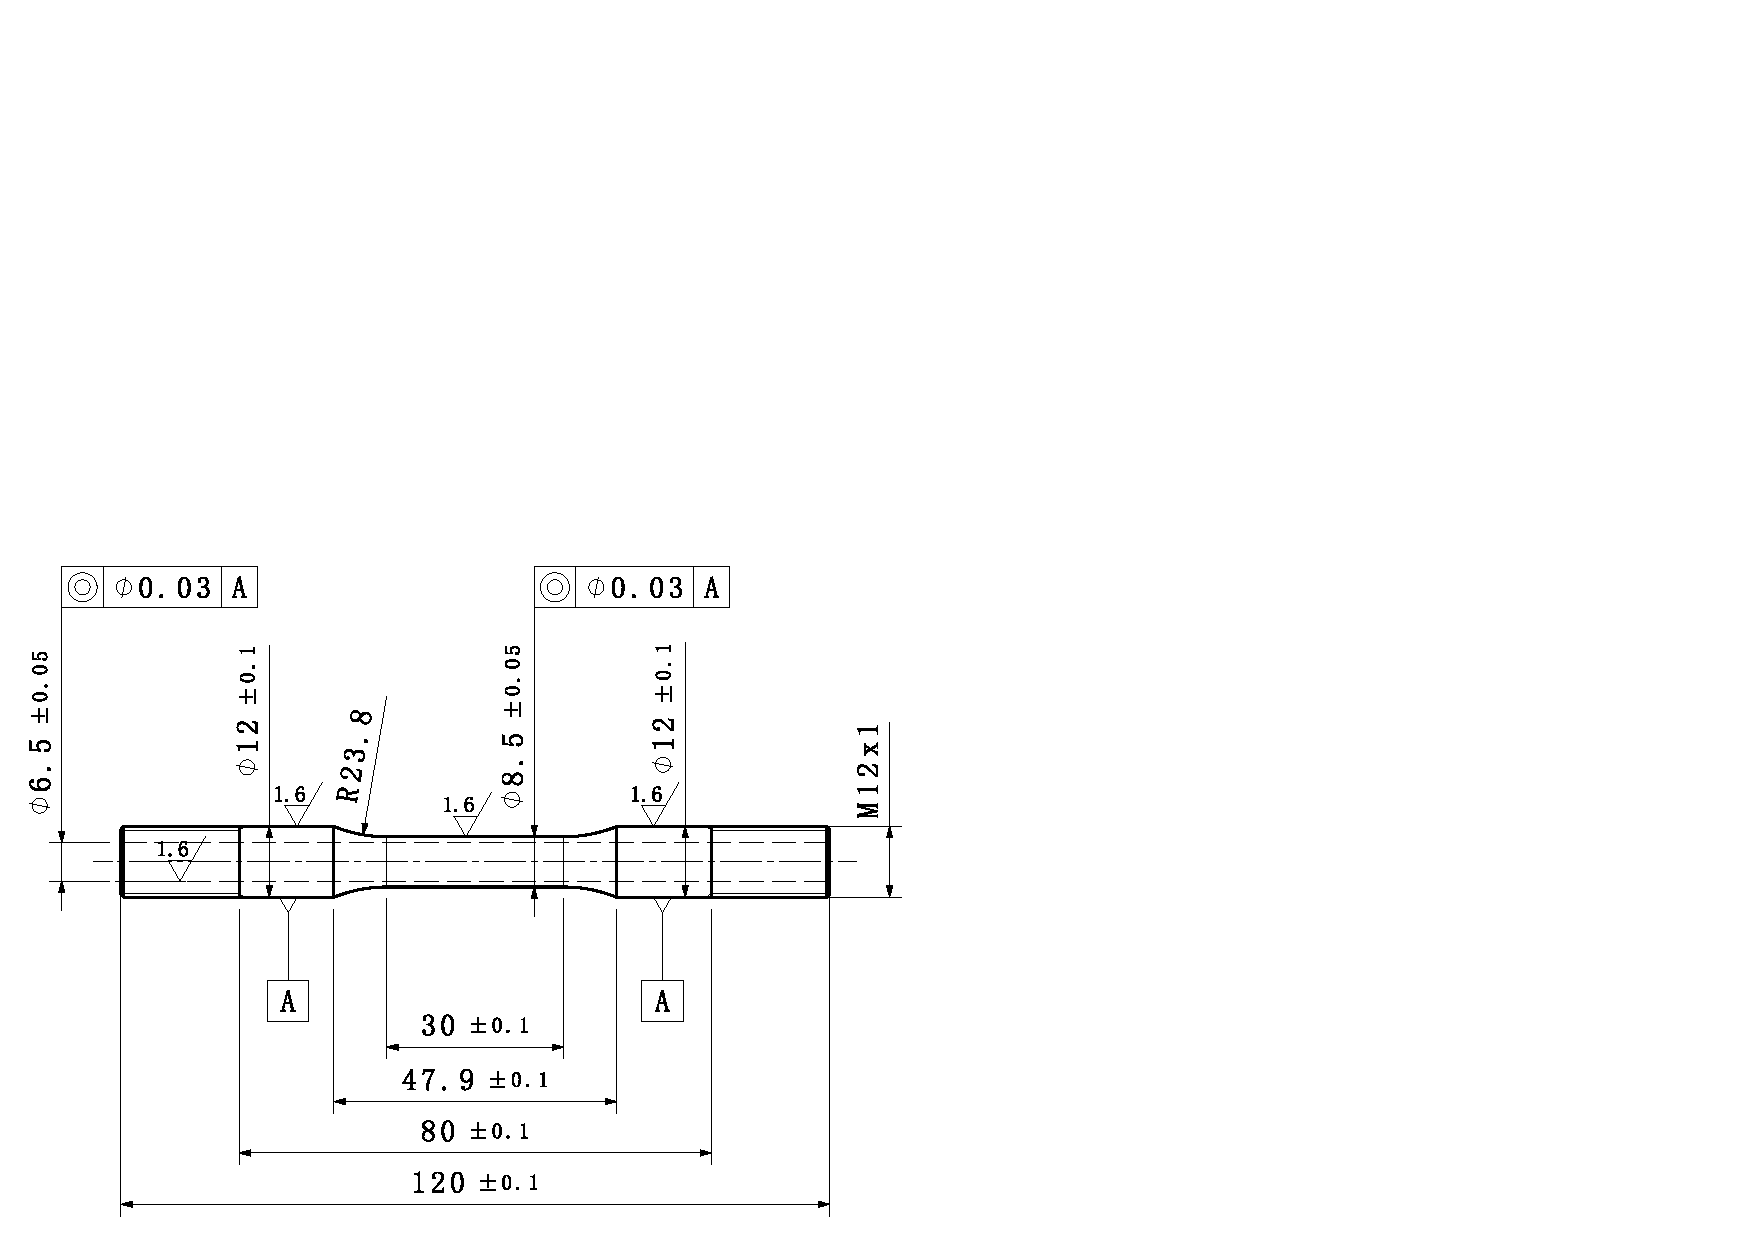
\includegraphics[width=8cm]{IN718_Axial_Specimen_TGMF.pdf}}
\caption{Dimensions of the specimen for TGMF testing.}
\label{Fig:IN718_Axial_Specimen_TGMF}
\end{figure}

\subsection{TGMF testing system}
The TGMF testing system for the thin-walled tubular specimen is shown in \autoref{Fig:tgmf_testing}. The testing system includes multiple subsystems such as loading, heating, air cooling, and water cooling. These subsystems work cooperatively to ensure the mechanical load and temperature over the specimen gauge section are simultaneously varied and independently controlled. 
\begin{figure}[!htp]
\centering{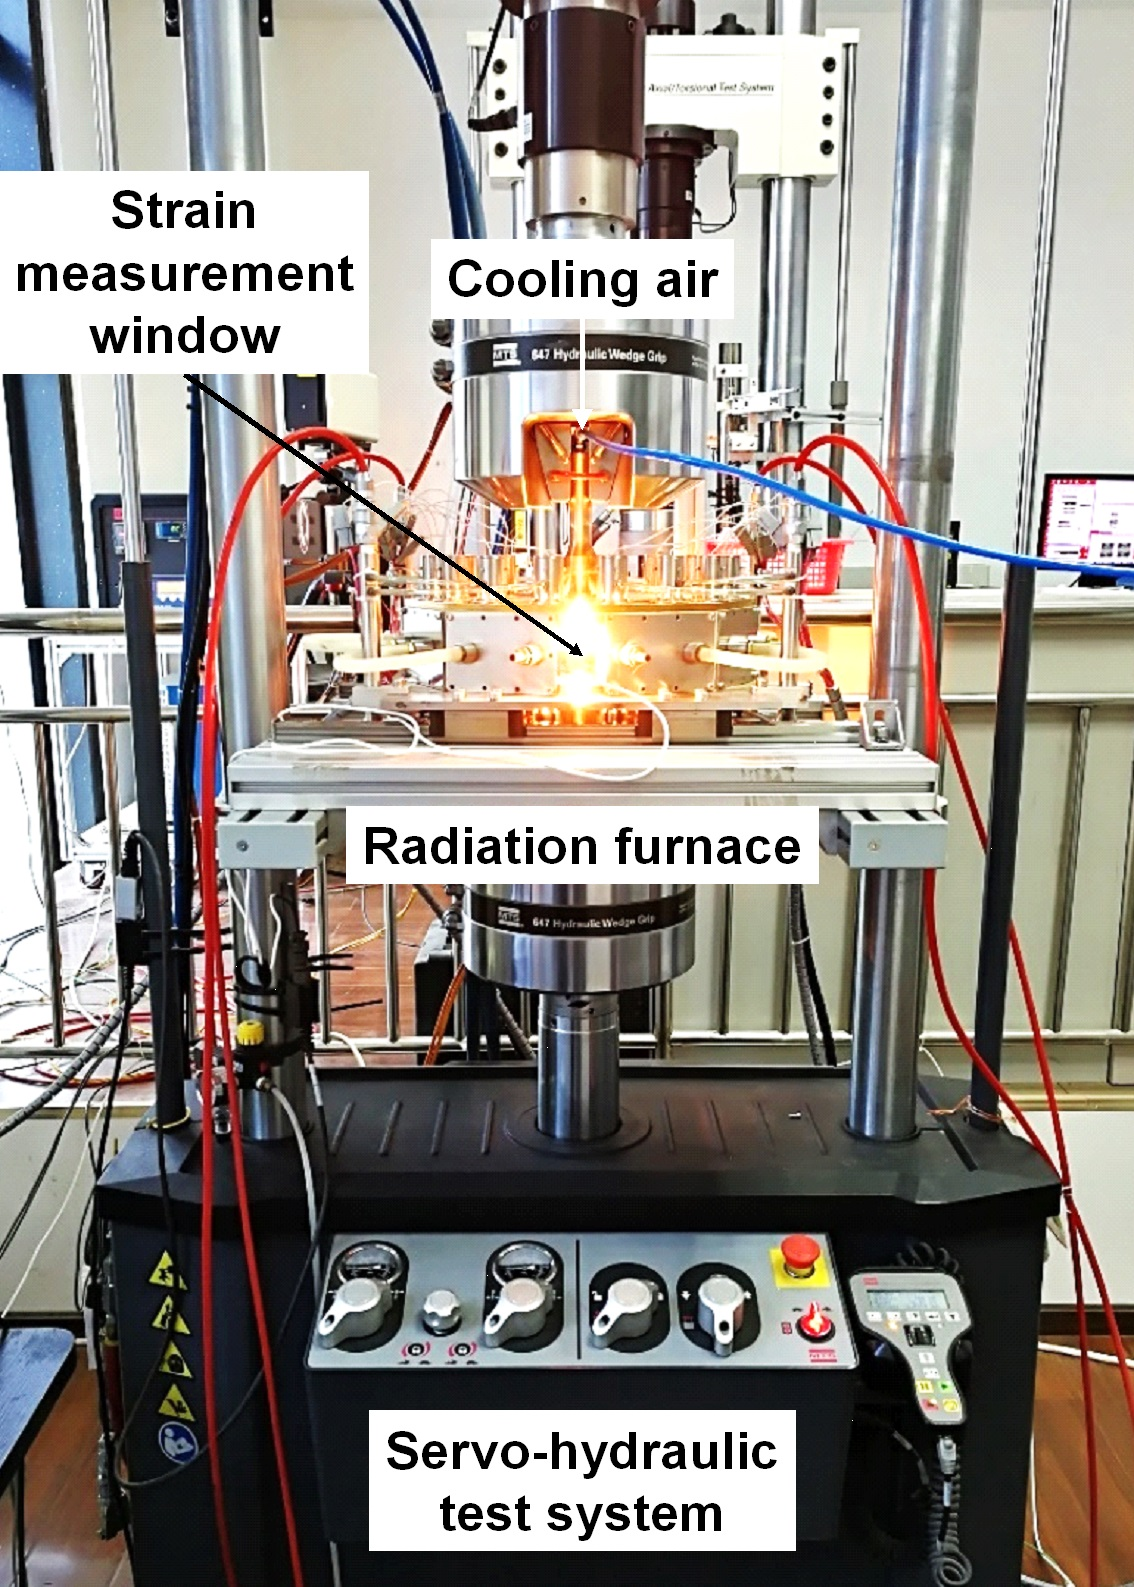
\includegraphics[height=12.0cm]{tgmf_testing.jpg}}
\caption{Experimental apparatus of TGMF test system.}
\label{Fig:tgmf_testing}
\end{figure}
% \begin{figure*}[!htp]
% 	\centering
% 	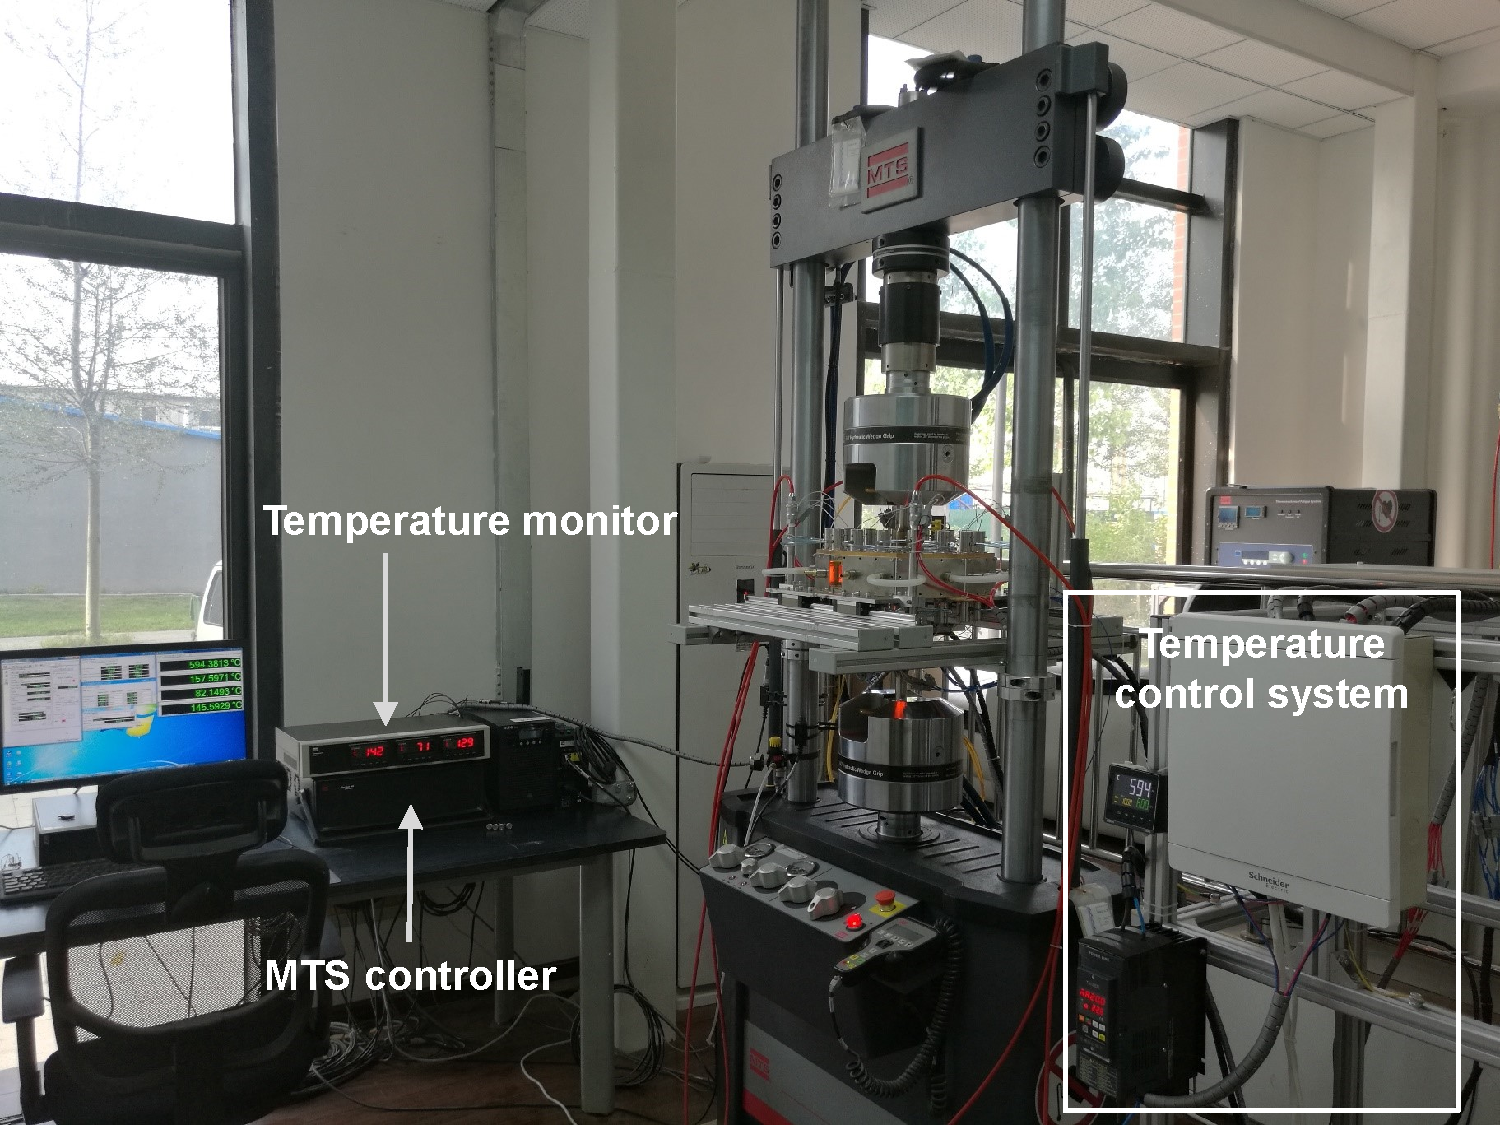
\includegraphics[width=12cm]{TGMF_Test_System.pdf}
% 	\caption{Experimental apparatus of TGMF test system.}
% 	\label{Fig:TGMF_Test_System}
% \end{figure*}

A MTS hydraulic servo fatigue test machine was used to apply a tension/compression mechanical load. The mechanical load is transmitted to the specimen through a fixture. As shown in \autoref{Fig:cooling}, the cooling air can enter the internal of the tubular specimen through the fixture. In order to reduce the additional bending moments and the bending stress in the specimen, the fixture must provide a sufficiently high degree of coaxiality. Meanwhile, the frame of the MTS testing system provides an alignment device, and it can effectively reduce the additional bending moments in the specimen during the test. The total strain is measured by a extensometer with a gauge length of 10 mm and a measuring range of $\pm$20\%. 

\begin{figure}[!htp]
	\centering
	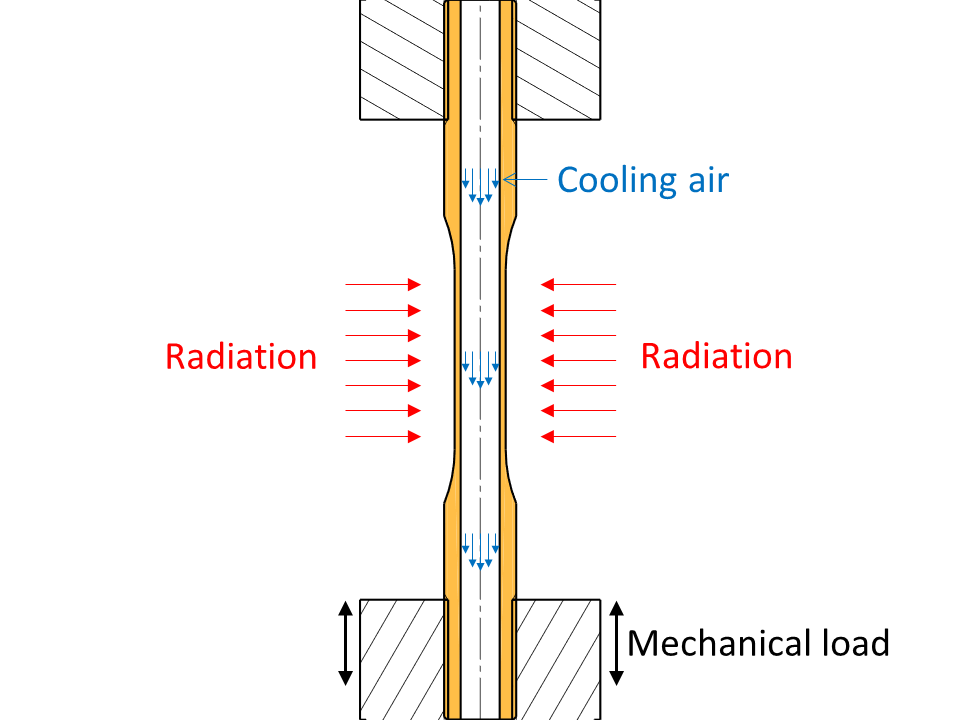
\includegraphics[width=8.0cm]{cooling.png}
	\caption{Locations of the temperature monitors.}
	\label{Fig:cooling}
\end{figure}

The temperature of the specimen was measured by the thermocouples. In practice, the choice of the diameter of the thermocouple wire is significant. A thick thermocouple wire will cause a delay in the temperature measurement. It leads to a temperature deviation between the thermocouple and the specimen, and it affects the response of the feedback control system. In order to improve the accuracy of temperature measurement and increase the response speed of thermocouples, the diameter of the thermocouple wire should be as smaller as possible. Therefore, the thermocouple wires with the diameter of 0.25 mm were used.

The temperature controller was used to control the temperature of the specimen.
The controller accepted the temperature sensor (thermocouple or infrared thermometer) as input and compare the actual temperature to the desired control temperature. It will then provide an output to the power regulator to control the luminance of the lamps. 
The temperature controller of the radiation furnace is a proportional–integral–derivative (PID) controller. The values of proportional, integral, and derivative gains of the PID controller can be determined by the PID tuning process.
However, the emissivity of the specimen and the temperature range will influence the PID gains of the temperature controller. Therefore, the PID gains should be tuned when the specimen surface was fully oxidized.

The air cooling subsystem consists of two air compressors, an air dryer, metering valves, air pressure gauges and cooling passages. 
The two air compressors were used to provide the cooling air of the specimen and the lamp holders, separately.
Each air compressor has a power of 2.4 kW and provides the compressed air of 0.4 - 0.8 MPa. The compressed air with a pressure of 0.7 MPa is filtered through the air dryer and output to the metering valve. The air dryer is used for removing water vapor from the compressed air.
During all of the TGMF tests, the pressure and the volume flow of the compressed air were kept as constants as 40 l/min. The metering valve was used to control the volume flow of the compressed air.
The air cooling subsystem also provides compressed air for the lamp holders.
The duration of the TGMF test is usually long, so the lamp holders have to be cooled to ensure that they can work properly.

% \begin{figure}[!htp]
% \centering{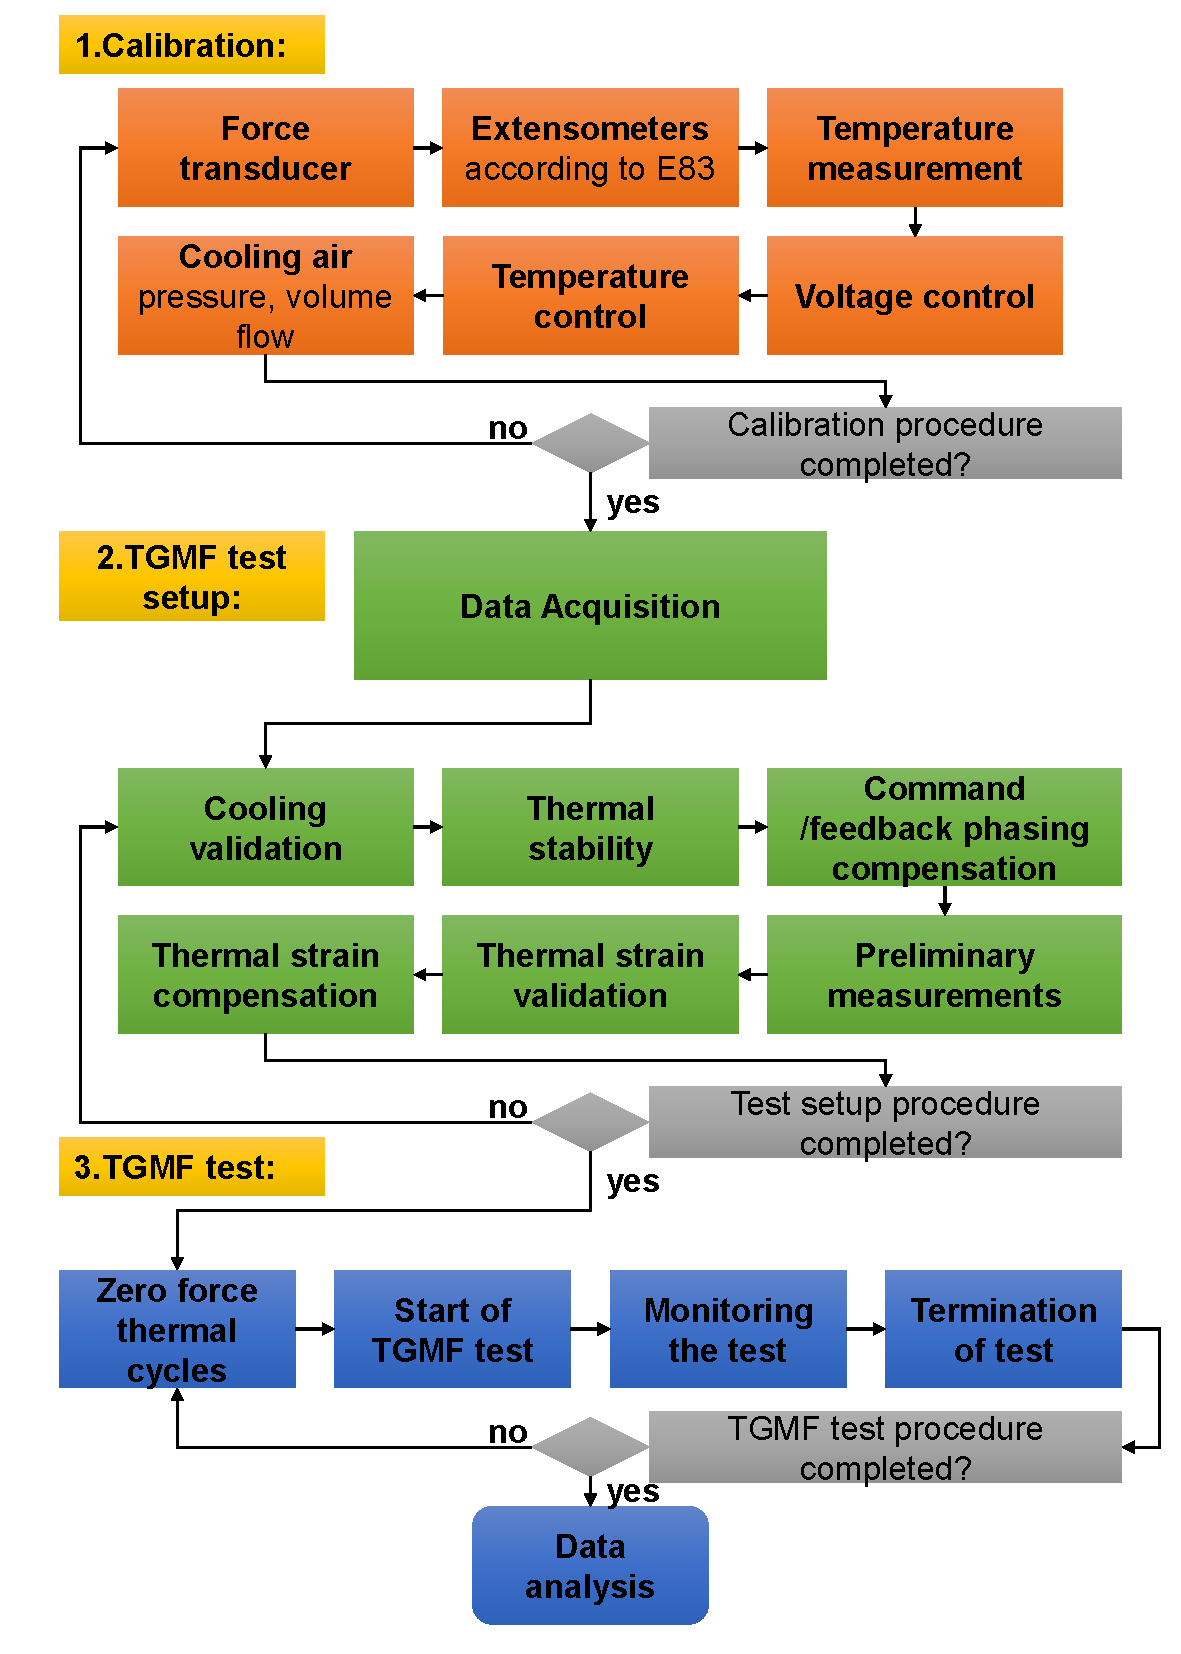
\includegraphics[height=12.0cm]{tgmf_code.pdf}}
% \caption{The experimental procedures of thermal gradient mechanical fatigue test.}
% \label{Fig:tgmf_code}
% \end{figure}


Recently, there are no relevant standards for TGMF testing. Because of the test processes of the TGMF and TMF are very similar, according to the testing process of TMF, the concepts in TGMF testing are defined as same as them in the TMF testing, such as:

\begin{itemize}
  \item {Thermal strain}, $\varepsilon_{\rm{th}}$,
  \item {Mechanical strain}, $\varepsilon_{\rm{mech}}$,
  \item {Total strain}, $\varepsilon_{\rm{tot}}=\varepsilon_{\rm{mech}}+\varepsilon_{\rm{th}}$,
  \item {Loading ratio}, $R_{\varepsilon}=\varepsilon_{\rm{mech,min}}/\varepsilon_{\rm{mech,max}}$,
  \item {Phase angle of the thermal loading and mechanical loading}, $\theta_{T-\varepsilon}$.
\end{itemize}

% According to the standards discussed above, 

% The implemented steps of the strain-controlled TGMF testing is shown in \autoref{Fig:tgmf_code}, in the form of a flow diagram.

\begin{figure}[!htp]
	\centering
	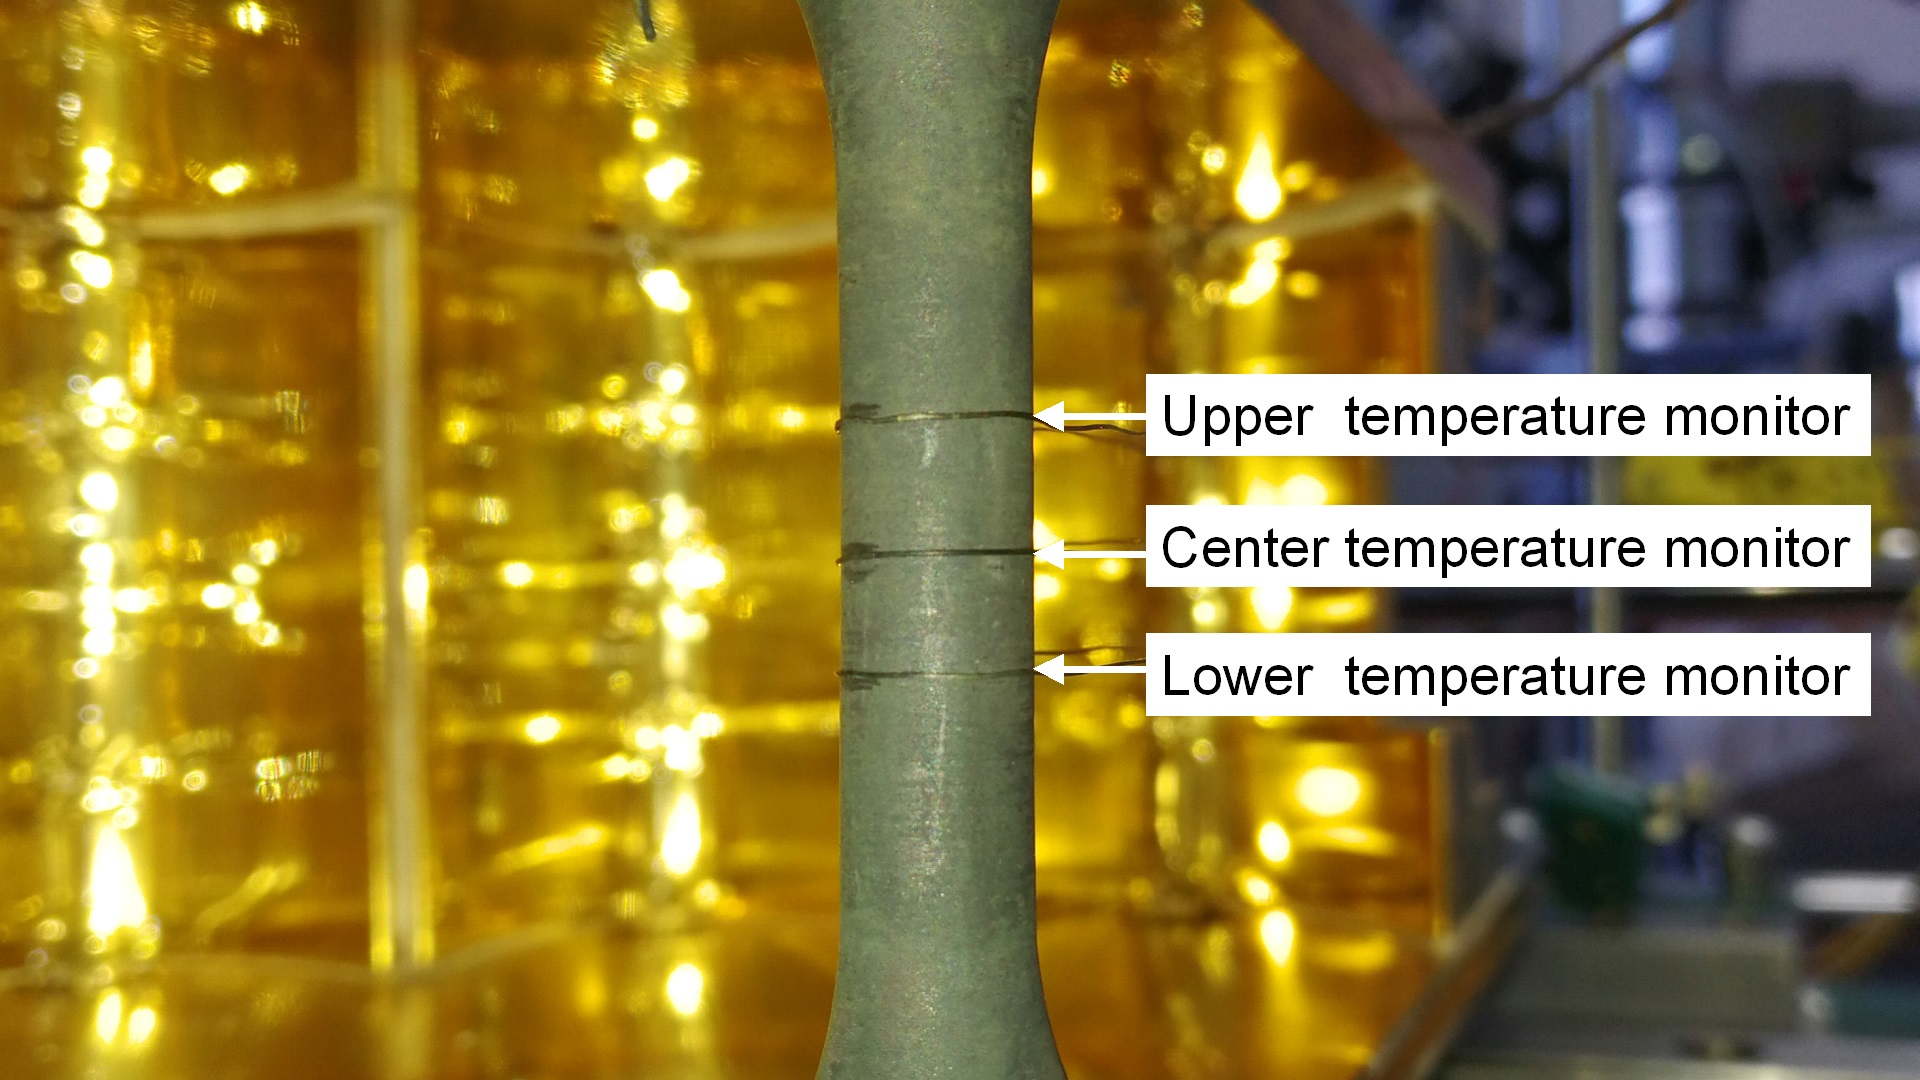
\includegraphics[width=8.0cm]{temperature_monitors_tgmf.jpg}
	\caption{Locations of the temperature monitors.}
	\label{Fig:temperature_monitors_tgmf}
\end{figure}



\begin{figure}[!htp]
	\centering
	\begin{overpic}[width=8.0cm]{plot_thermal_stability_tgmf.pdf}
		\put(84,65){\fcolorbox{white}{white}{(a)}}
	\end{overpic}
	\begin{overpic}[width=8.0cm]{plot_thermal_stability_tgmf_deviation.pdf}
		\put(84,65){\fcolorbox{white}{white}{(b)}}
	\end{overpic}
	\caption{Varying temperatures in a tubular specimen with the gauge length of 15 mm, heated by the radiation furnace. (a) Temperature variations of three thermal elements during a loading cycle. (b) Temperature deviations in the axial direction.}
	\label{Fig:thermal_stability_TGMF}
\end{figure}

The light reflected on the upper and lower gold-coated walls leads to the highest intensity of radiation in the middle section of the specimen.
This will cause a temperature gradient along the axial direction of the specimen, and the highest temperature will occur at the middle section of the specimen during the TGMF test.
Unlike the induction heating, the axial temperature gradient of the specimen is difficult to adjust by modifying the radiation furnace.
Therefore, the influence of the axial temperature gradients has to be considered in the computation.

In order to obtain the temperature distribution of the specimen during the TGMF testing, temperatures at the upper, center and lower positions in the gauge section of the specimen were measured by the thermocouples wrapped around the specimen. \autoref{Fig:temperature_monitors_tgmf} shows the locations of the thermocouples. In the study, the temperature range of the TGMF testing is from 300$^\circ$C to 650$^\circ$C. The cycle period was predetermined as 240 s with a triangular shape temperature cycle, thus the heating and cooling rates were about 2.2$^\circ$C/s.
\autoref{Fig:thermal_stability_TGMF}(a) shows the dynamic temperature measurement during a stable TGMF cycle and \autoref{Fig:thermal_stability_TGMF}(b) shows the temperature deviations between each thermocouple and the temperature command.
It is observed that the maximum axial temperature gradients during the TMF test are less than $\pm30$$^\circ$C.





% Conventional thermomechanical fatigue tests are not able to simulate these stress conditions and achieve a temperature gradient in the radial direction. So we designed this test system for thermal gradient mechanical fatigue (TGMF) testing.
% The system can realize the controlled thermal cycle with temperature gradient on the hollow specimen and apply the mechanical load at the same time.
% The external surface of the specimen is heated by the method of concentrating radiation, while the inner surface is cooled by compressed air to achieve the temperature gradient.
% The test system needs to achieve high heating and cooling speed, so the power of heating system and the volume flow of the cooling air should be designed in detail.

\section{Experimental results of TGMF tests}

The experimental conditions and results of IF, TMF and TGMF tests are summarized in \autoref{Tab:test_matrix_TGMF}. The isothermal fatigue (IF) tests were performed at 650$^\circ$C, and the in-phase thermomechanical fatigue (TMF-IP) and the out-of-phase thermomechanical fatigue (TMF-OP) tests were carried out with a temperature range of 300–650$^\circ$C, as introduced in Refs. \cite{SUN2019228, SUN201989}. In order to compare with the TMF testing results, the TGMF tests with the same temperature range of 300–650$^\circ$C and two kinds of phase angles were carried out: 0$^\circ$ (IP) and 180$^\circ$ (OP). Each kind of TGMF tests was conducted with four or five different mechanical strain amplitudes. The load type TGMF-IP is short for the tension-compression in-phase thermal gradient mechanical fatigue, and TGMF-OP means the tension-compression out-of-phase thermal gradient mechanical fatigue. The nickle-based superalloy Inconel 718 used in Refs. \cite{SUN2019228, SUN201989} were as same as the superalloy used in this study, therefore it is reasonable to compare the fatigue lifetime of these tests.
% The abbreviation TBC means the specimen is covered with the thermal barrier coating.
Because of the thermal gradients in radial and axial directions, the axial stress is not constant on the cross-section of the specimen.
Therefore, the stress distribution of the specimen during the test has to be obtained by the finite element method.
In order to facilitate the comparison and analysis between the computational and experimental results, the nominal axial stress $\sigma$ on the cross section is used in the following figures, and it is given by,
\[\sigma = F/A.\]
% 图\autoref{Fig:plot_exp_TCTGMF}(a),(c)分别是同相位和反相位热梯度机械疲劳的稳定滞后回线。
% 由于热梯度机械疲劳的温度循环与载荷循环之间有相位差,导致其拉伸半周和压缩半周具有不同的循环软化行为。
% 对于同相位热梯度机械疲劳试验,合金在拉伸半周表现出较强的循环软化,而对于反相位热梯度机械疲劳试验则相反,合金在压缩半周表现出较强的循环软化。

\autoref{Fig:plot_exp_TCTGMF}(a) and (c) show the stable hysteresis loops of TGMF tests under IP and OP loading conditions, respectively.
Since there is a phase difference between the temperature cycle and the load cycle of the thermal gradient mechanical fatigue, the tensile half cycle and the compression half cycle have different cycle softening behaviors.
For the TGMF-IP test, an evident cyclic softening was observed during the tensile half-cycle, whereas for the TGMF-OP test, the alloy performed a significant cyclic softening during the compression half-cycle.

% 如果是右对齐,那么只需要将\centering换成\raggedleft,如果左对齐,那么换成\raggedright即可。
\begin{table}[htbp]
  \centering
  \caption{Experimental conditions and results of thermal gradient mechanical fatigue tests.}
    \begin{tabular}{p{2.0cm}p{1.0cm}<{\centering}p{2cm}<{\centering}p{0.6cm}<{\centering}p{1.2cm}<{\raggedleft}}
    \toprule
    Test Type & $\pm \varepsilon _{\rm{mech}}$ & $\dot \varepsilon _{\rm{mech}}$ & $\theta_{\rm{T-\varepsilon}}$ & $N_{\rm{f}}$ \\
          & [\%]  & [s$^{-1}$] & [$^\circ$] & [cycle] \\
    \midrule
    IF \cite{SUN2019228} & 1.00  & $1\times 10^{-3}$ & -  & 231 \\
          & 0.80  & $1\times 10^{-3}$ & -  & 326 \\
          & 0.70  & $1\times 10^{-3}$ & -  & 592 \\
          & 0.60  & $1\times 10^{-3}$ & -  & 1336 \\
          & 0.50  & $1\times 10^{-3}$ & -  & 8449 \\
          & 0.45  & $1\times 10^{-3}$ & -  & 15497 \\
          & 0.40  & $6.4\times 10^{-3}$ & -  & 130585 \\
    \midrule
    TMF-IP  & 1.00 & $2.22\times 10^{-4}$ & 0   & 58 \\
    \cite{SUN2019228}      & 0.80 & $1.78\times 10^{-4}$ & 0   & 176 \\
          & 0.70 & $1.56\times 10^{-4}$ & 0   & 248 \\
          & 0.60 & $1.33\times 10^{-4}$ & 0   & 1297 \\
    \midrule
    TMF-OP  & 1.00 & $2.22\times 10^{-4}$ & 180 & 209 \\
    \cite{SUN2019228}      & 0.80 & $1.78\times 10^{-4}$ & 180 & 303 \\
          & 0.70 & $1.56\times 10^{-4}$ & 180 & 429 \\
          & 0.65 & $1.44\times 10^{-4}$ & 180 & 633 \\
    \midrule
    TGMF-IP & 0.80  & $1.67\times 10^{-4}$ & 0     & 48 \\
          & 0.70  & $1.33\times 10^{-4}$ & 0     & 50 \\
          & 0.60  & $1.22\times 10^{-4}$ & 0     & 107 \\
          & 0.50  & $1.11\times 10^{-4}$ & 0     & 208 \\
          & 0.425  & $0.89\times 10^{-4}$ & 0     & 1066 \\
    \midrule
    TGMF-OP & 0.80  & $1.67\times 10^{-4}$ & 180   & 128 \\
          & 0.60  & $1.22\times 10^{-4}$ & 180   & 375 \\
          & 0.50  & $1.11\times 10^{-4}$ & 180   & 864 \\
          & 0.425  & $0.89\times 10^{-4}$ & 180   & 3387 \\
    \bottomrule
    \end{tabular}%
  \label{Tab:test_matrix_TGMF}%
\end{table}%

\begin{figure*}[!htp]
  \centering
  \begin{overpic}[width=8.0cm]{plot_exp_half_life_cycle_TCIPTGMF.pdf}
    \put(84,13){\fcolorbox{white}{white}{(a)}}
  \end{overpic}
  \begin{overpic}[width=8.0cm]{plot_exp_pv_TCIPTGMF.pdf}
    \put(84,13){\fcolorbox{white}{white}{(b)}}
  \end{overpic}

  \begin{overpic}[width=8.0cm]{plot_exp_half_life_cycle_TCOPTGMF.pdf}
    \put(84,13){\fcolorbox{white}{white}{(c)}}
  \end{overpic}
  \begin{overpic}[width=8.0cm]{plot_exp_pv_TCOPTGMF.pdf}
    \put(84,13){\fcolorbox{white}{white}{(d)}}
  \end{overpic}

  \caption{Experimental results of TGMF tests with varying temperature between 300$^\circ$C and 650$^\circ$C. Noting that, the vertical axis axial stress $\sigma$ is the nominal stress.
  (a) Half life stable hysteresis loops of TGMF-IP tests.
  (b) Peak and valley stresses of TGMF-IP tests.
  (c) Half life stable hysteresis loops of TGMF-OP tests.
  (d) Peak and valley stresses of TGMF-OP tests.}
  \label{Fig:plot_exp_TCTGMF}
\end{figure*}

\begin{figure}[!htp]
  \centering{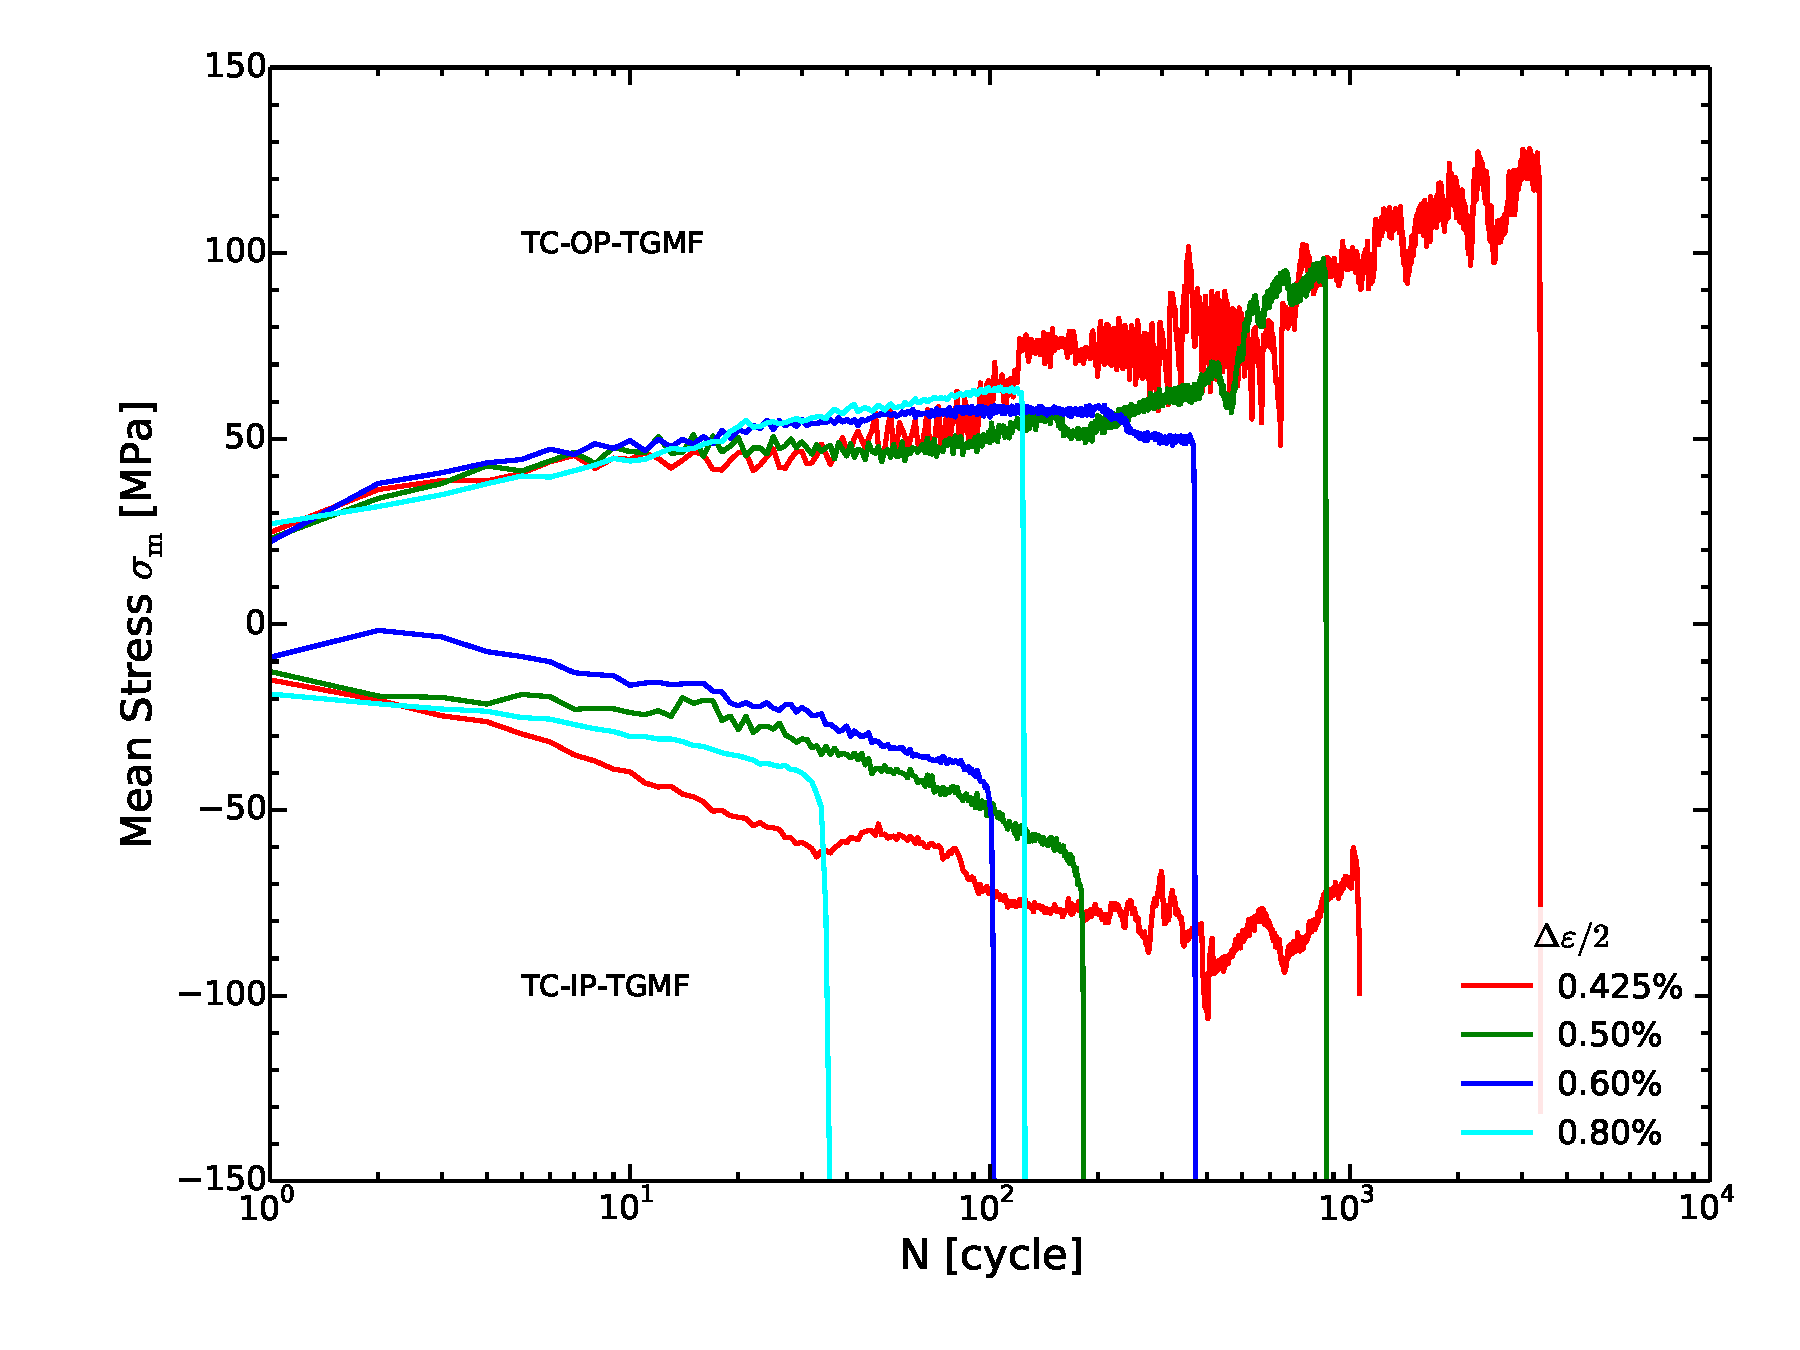
\includegraphics[width=8cm]{plot_exp_mean_TCTGMF.pdf}}
  \caption{The evolution of mean stresses under TMF-IP-TGMP and TMF-OP-TGMP loading conditions.}
  \label{Fig:plot_exp_mean_TCTGMF}
\end{figure}

% 图\autoref{Fig:plot_exp_TCTGMF}(b),(d)分别是同相位和反相位热梯度机械疲劳的循环应力峰谷值和均值。
% 在所有的试验条件下,合金在最终断裂前循环应力峰谷值快速下降,这实际上是宏观裂纹的形成以及随后的失稳扩展至断裂的结果。
% 同相位和反相位热梯度机械疲劳试验均表现为循环软化,但温度循环与载荷循环之间的相位差,导致循环软化的程度不同,在300-650$^{\circ}$C范围内,温度越高,材料的循环软化越明显,因此对于同相位的情况,材料在拉伸半周的循环软化更强烈,反应在平均应力的演化上则表现为平均应力随着循环的增加,产生越来越大的平均压应力。
\autoref{Fig:plot_exp_TCTGMF}(b), (d) illustrate the peak, valley and mean values of the stress response of the TGMF-IP and TGMF-OP tests, respectively.
Under both experimental conditions, the peak and valley value of the cyclic stress drops rapidly before the final fracture, which is caused by the cracks propagate and reach the critical crack size.
Cyclic softening were observed during both in-phase and out-of-phase thermal gradient mechanical fatigue tests, but the phase difference between the temperature cycle and the load cycle leads to the different cycle softening behavior. In the temperature range of 300$^\circ$C to 650$^\circ$C, the higher the temperature, the more obvious the cyclic softening of the material. Therefore, under TGMF-IP loading condition, the cyclic softening of the superalloy in the tensile half-cycle is more evident, whereas, under TGMF-OP loading condition, the cyclic softening behavior was observed more evident in the compression half-cycle. The asymmetry of cyclic softening in tension and compression results in an evolution of the mean stress during the fatigue test.

% 平均应力是高温低周疲劳中不可忽视的因素,尤其对于强度较高而韧性较低的镍基高温合金而言,平均应力是影响疲劳寿命的重要因素,图\autoref{Fig:plot_exp_mean_TCTGMF}所示为Inconel 718合金在同相位和反相位TGMF试验条件下的平均应力响应曲线。可见,对于TGMF-IP,平均应力为压应力,机械应变幅的增加对平均应力的影响不大,对于不同的机械应变幅值,平均应力演化的速率相近,平均应力的数值随着循环数的增加而增大,
The mean stress is a factor that can not be ignored in low-cycle fatigue. Especially for nickel-based superalloys with high strength and low toughness, the mean stress is an important factor affecting the fatigue life, as shown in \autoref{Fig:plot_exp_mean_TCTGMF}. The mean stress response curve for the Inconel 718 alloy under the in-phase and reverse phase TGMF test conditions. It can be seen that for TGMF-IP, the mean stress is compressive stress, and the increase of the mechanical strain amplitude has little effect on the mean stress. For different mechanical strain amplitudes, the mean stress evolution rate is similar, and the mean stress value increases with the number of cycles.

% ,当$\Delta_{\varepsilon}=0.4\%$时,半寿命时的压缩平均应力为66.7MPa。对于TGMF-OP,平均应力为拉应力且随着机械应变幅的增加拉伸平均应力幅度变大,当$\Delta_{\varepsilon}=0.4\%$时,半寿命时的拉伸平均应力约为52.3MPa。
For TGMF-OP test, the mean stress becomes a tensile stress and the tensile stress increased with the increase of the mechanical strain amplitude.
When $\Delta \varepsilon=0.8\%$, the mean stress at the half-life cycle is about 50 MPa. For TGMF-IP test, the mean stress becomes a compression stress. When $\Delta \varepsilon=0.8\%$, the mean stress at the half-life cycle is about -30 MPa.

% TGMF中存在明显平均应力的原因是合金的强度随温度的不断变化,无论是同相位还是反相位热梯度机械疲劳都经历低温到高温的温度循环,当试验温度较高时合金的强度较低,而当试验温度较低时合金的强度较高,因此造成了滞后回线的应力不对称性,平均应力总是偏向低温半周,而平均应力随机械应变幅增加而增大的原因是随着机械应变幅的增加,合金在高温半周产生的塑性变形增加,这加剧了拉压应力的不对称性。此外,可以观察到在两种TGMF试验条件下平均应力幅值均随循环的进行而逐渐增大,这可认为是IN718合金在高温半周循环软化更为强烈的结果。等温疲劳试验,平均应力数值普遍较小,因此平均应力对等温疲劳试验的影响可以忽略。
The evolution of mean stress in TGMF is that the strength of the alloy changes with temperature. Both in-phase and out-of-phase TGMF tests, temperature cycles in the temperature interval of 300$^\circ$C to 650$^\circ$C. When the temperature is high, the strength of the alloy is low. On the contrary, when the temperature is low, the strength of the alloy becomes high. It results in the stress asymmetry of the hysteresis loop. The mean stress is always towards to the low-temperature half cycle.
The reason is that with the increase of the mechanical strain amplitude, the plastic deformation of the alloy at the high-temperature half cycle increases, which aggravates the asymmetry of tensile and compressive stress.
Besides, it can be observed that the absolute values of the mean stresses increase gradually with the cycling in TGMF loading conditions, which can be considered as a result of the more intense softening of the superalloy Inconel 718 during the high-temperature half cycle. In the isothermal fatigue test, the mean stress value is generally small, so the mean stress has a negligible effect on the isothermal fatigue test.

\begin{figure}[!htp]
\centering{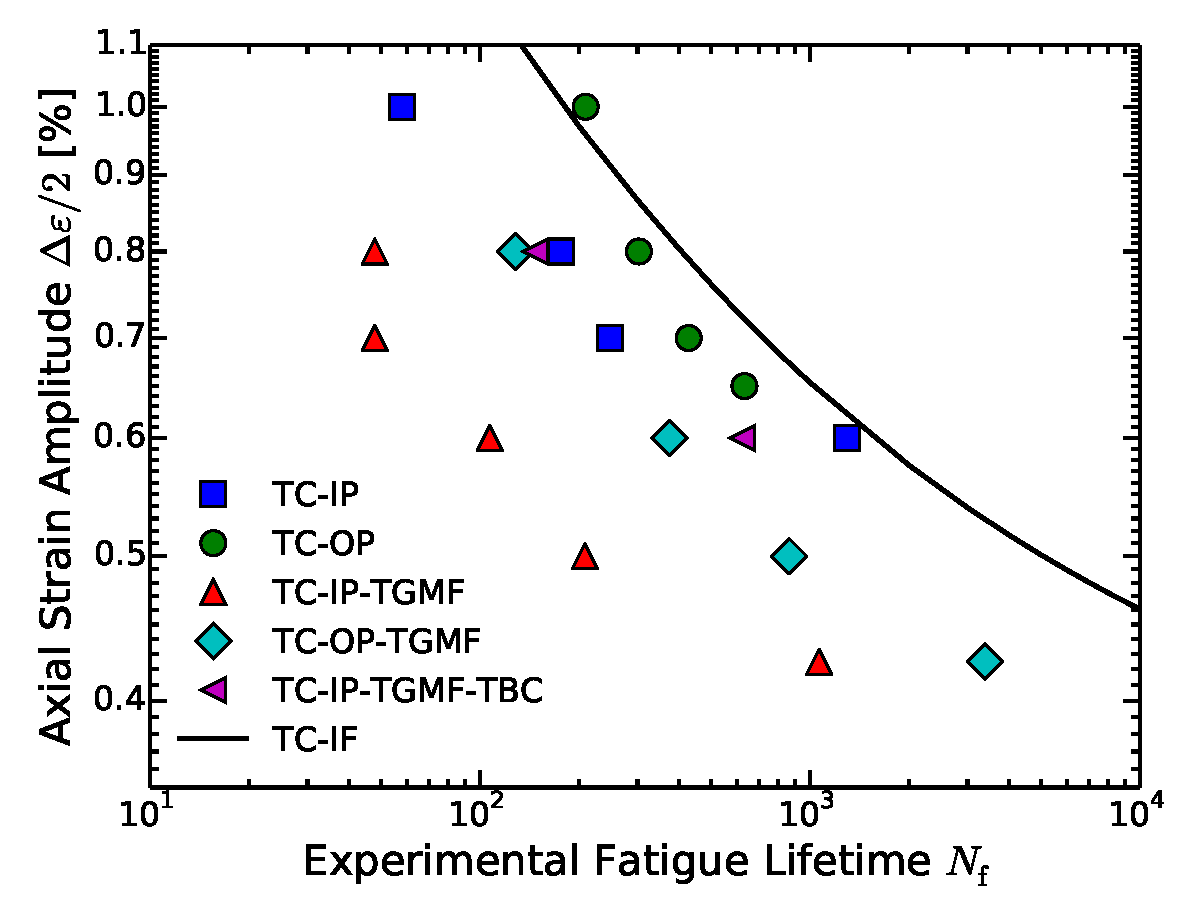
\includegraphics[width=8cm]{plot_exp_fatigue_life_TGMF.pdf}}
\caption{Comparison of the fatigue lives under IF, TMF and TGMF loading conditions.}
\label{Fig:plot_exp_fatigue_life_TGMF}
\end{figure}

% 在机械应变控制条件下,一般可以通过机械应变幅与疲劳寿命之间的关系来考查材料的热机械疲劳寿命行为。图\autoref{Fig:plot_exp_fatigue_life_TGMF}所示为300-650$^{\circ}$C同相位、反相位热机械疲劳和热梯度机械疲劳试验条件下机械应变与疲劳寿命之间的关系,图中黑色实线为650$^{\circ}$C等温疲劳的Coffin-Masson疲劳寿命曲线。可见300-650$^{\circ}$C的热机械疲劳与热梯度机械疲劳比650$^{\circ}$C等温疲劳具有更大的损伤。在同等机械应变幅下650$^{\circ}$C等温低周疲劳具有较高的疲劳寿命。
% 对于热机械疲劳(TMF),同相位和反相位试验的机械应变幅-寿命关系曲线存在相互交叉,交叉点的位置大概在机械应变幅为0.6\%左右。
% 当机械应变幅较高时,同相位热机械疲劳倾向于具有较低的疲劳寿命而当机械应变幅较低时,反相位热机械疲劳倾向于具有较低的疲劳寿命。
% 而对于热梯度机械疲劳(TGMF),同相位和反相位试验的机械应变幅-寿命关系曲线并没有存在相互交叉的趋势,同相位热梯度机械疲劳一直具有较低的疲劳寿命。

Under mechanical strain control, the fatigue life can generally be examined by the relationship between mechanical strain amplitude and fatigue life.
\autoref{Fig:plot_exp_fatigue_life_TMF_TGMF_TC} shows the comparison of the fatigue lifetimes of TMF and TGMF tests under in-phase and out-of-phase loading conditions, respectively.
The TGMF-IP life is smaller than the TMF-IP life, as shown in \autoref{Fig:plot_exp_fatigue_life_TMF_TGMF_TC}(a) and the TGMF-OP life is smaller than the TMF-OP life, as shown in \autoref{Fig:plot_exp_fatigue_life_TMF_TGMF_TC}(b).
The temperature cycles of the TMF and TGMF tests are the same, the only difference between the TMF and TGMF tests is the temperature gradient in the specimen.
Therefore, the temperature gradient is considered to have a significant effect on the fatigue life under the thermomechanical loading condition.
Comparing \autoref{Fig:plot_exp_fatigue_life_TMF_TGMF_TC}(a) with \autoref{Fig:plot_exp_fatigue_life_TMF_TGMF_TC}(b), the reduction of TGMF-IP life due to the temperature gradient is more evident than the reduction of TGMF-OP life.

\begin{figure}
  \centering
  \begin{overpic}[width=8.0cm]{plot_exp_fatigue_life_IP.pdf}
    \put(84,65){\fcolorbox{white}{white}{(a)}}
  \end{overpic}
  \begin{overpic}[width=8.0cm]{plot_exp_fatigue_life_OP.pdf}
    \put(84,65){\fcolorbox{white}{white}{(b)}}
  \end{overpic}
  \caption{Comparison of fatigue lives of TMF and TGMF: (a) IP, (b) OP.}
  \label{Fig:plot_exp_fatigue_life_TMF_TGMF_TC}
\end{figure}

\section{Thermal gradient mechanical FE-analysis}

\subsection{Internal cooling of the specimen}

% TGMF试验的试件内表面采用压缩空气进行冷却,冷却系统的结构如图\autoref{Fig:inner_cooling}所示,包括空气压缩机、空气干燥器、流量计、压力表和流量控制器组成。
The internal surface of the specimen was cooled with the compressed air. The cooling system consists of the air compressor, air dryer, flow meter, pressure gauge and flow controller.
Because of the small inner diameter 6.5 mm of the specimen, it is difficult to measure the temperature of the specimen inner surface during the tests. 
A variety of measurement options were tried to measure the inner surface temperature.
It was found that the internal cooling air has a significant effect on the temperature measurement of the inner surface of the specimen.
% 内部冷却空气对试件内壁的温度测量有很大的影响。
The measured temperature is not the temperature of the inner surface, but the average temperature of the wall and the cooling air flow.
% 测量得到的温度不是壁面的温度,而是壁面和冷却气流的平均温度。
Therefore we tried to calculate the temperature distribution of the specimen inner surface using the finite element method.

% \begin{figure}[!htp]
% \centering{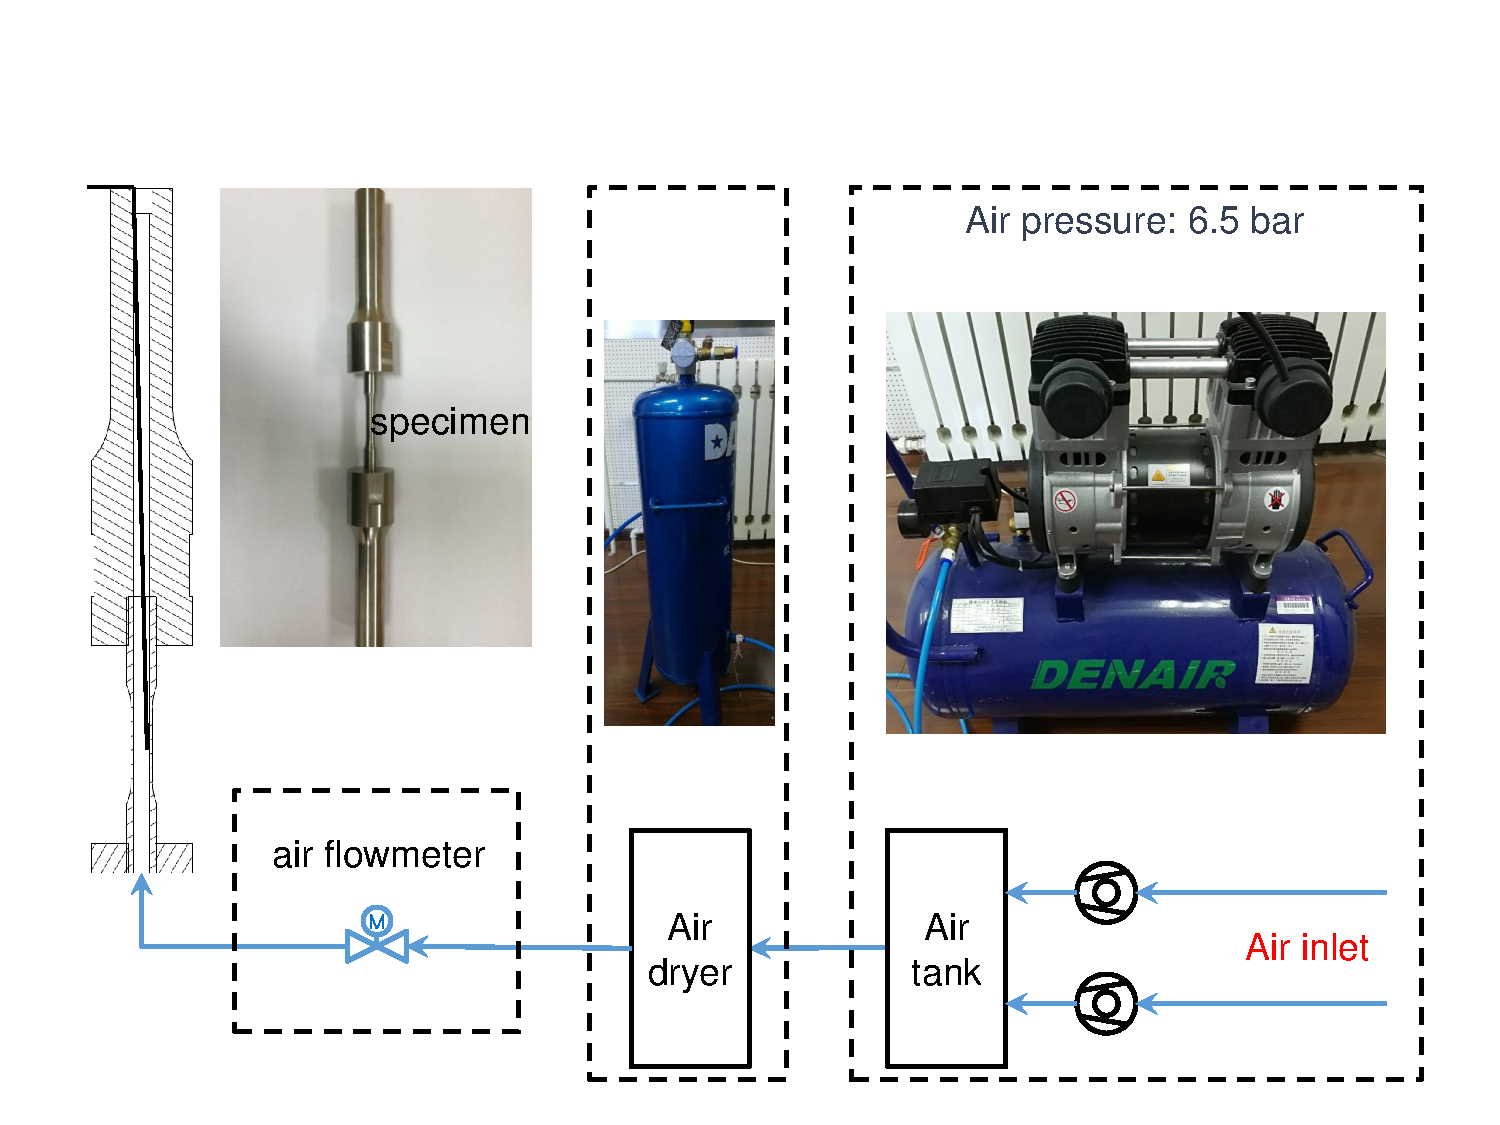
\includegraphics[width=8cm]{inner_cooling.pdf}}
% \caption{Schematic of inner cooling air system.}
% \label{Fig:inner_cooling}
% \end{figure}

\subsection{FE-model}

% TGMF试件的几何形状如图\autoref{Fig:Specimen}所示,由于几何形状和外部环境的对称性,我们取出试样的标距段部分,建立轴对称有限元模型,如图\autoref{Fig:FEM}所示,标距段长度为12mm,取试件的中心界面作为轴对称面。
% 用以下物理边界条件进行辐射加热的TGMF试样几何形状的有限元分析:
% 试件外表面为温度边界,随时间变化的温度分布可由试验测得,试件内表面为对流边界条件,对流换热系数由圆管强制对流换热公式计算,需要试验测量冷却空气的密度、温度和体积流量。由于试件的对称性,中心对称界面可假设为绝热边界,试件的上边界认为是热传导边界,对于热辐射,取试件表面的发射率为$\varepsilon=0.75$。
The geometry of the TGMF specimen is shown in \autoref{Fig:IN718_Axial_Specimen_TGMF}, because of the symmetry of the geometry and the external environment, we took out the gauge section of the specimen and created an axisymmetric finite element model. As shown in \autoref{Fig:FE_model}, the gauge length is 12 mm, and the center cross-section of the specimen is taken as the symmetric plane.
The outer surface of the specimen is defined as a temperature boundary condition. The temperature distribution of the outer surface was measured during the tests. The inner surface of the specimen is considered as a convection boundary condition. The convective heat transfer coefficient can be calculated by an empirical formula for turbulent flow in tubes. The density, temperature and volume flow of the cooling air need to be measured. The specimen is symmetric about its central cross-section. Therefore, only half of the specimen is modeled, and a symmetry boundary condition is applied.
The upper surface of the model is considered as a thermal conduction boundary. For radiation calculations, the emissivity of the surface of the specimen is defined as 0.75.

\begin{figure}[!htp]
  \centering{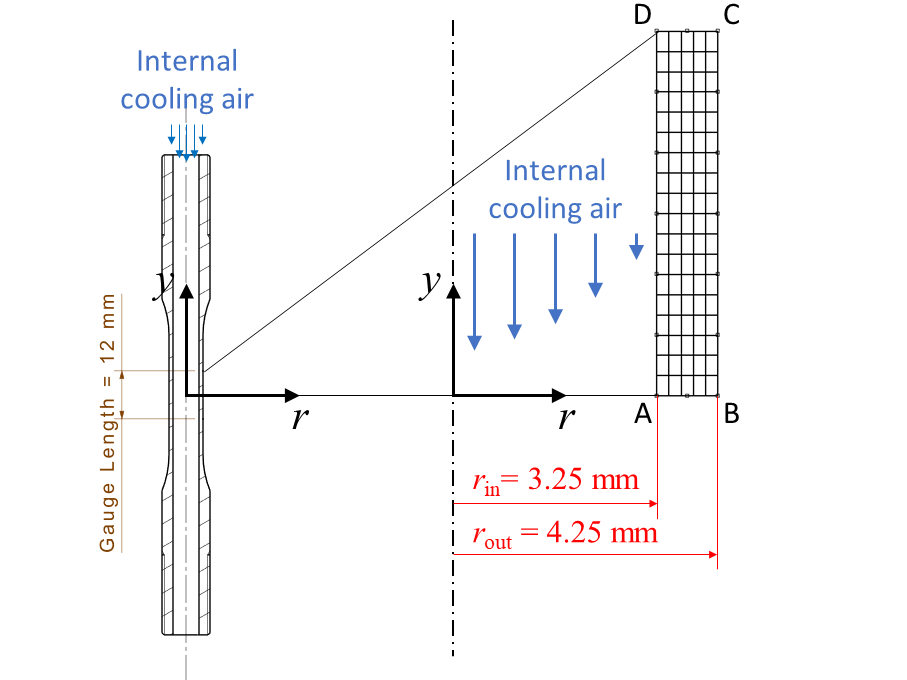
\includegraphics[width=9cm]{FE_model.png}}
  \caption{Schematic diagram of the finite element model.}
  \label{Fig:FE_model}
\end{figure}

\subsection{Forced convection in turbulent pipe flow}
The inner surface of the hollow specimen can be considered as a pipe.
%空心试件可以简化为圆管.
According to the formula of convection in turbulent pipe flow, the convective heat transfer coefficient of the inner surface of the specimen can be calculated.
%根据圆管内部的强制对流换热公式,我们计算试件内表面的对流换热系数。

Nusselt number (Nu) is a dimensionless number, defined as the ratio of convective to conductive heat transfer across (normal to) the boundary.
The Nusselt number is given as:
\[{\rm{N}}{{\rm{u}}_L} = \frac{{hL}}{k},\]
where $h$ is the convective heat transfer coefficient of the fluid, $L$ is the characteristic length, $k$ is the thermal conductivity of the fluid.

Gnielinski's correlation for turbulent flow in tubes is given as:
\[{\rm{N}}{{\rm{u}}_D} = \frac{{\left( {f/8} \right)\left( {{\rm{R}}{{\rm{e}}_D} - 1000} \right){\rm{Pr}}}}{{1 + 12.7{{(f/8)}^{1/2}}\left( {{\rm{P}}{{\rm{r}}^{2/3}} - 1} \right)}},\]
where $f$ is the Darcy friction factor that can either be obtained from the Moody chart or for smooth tubes from correlation developed by Petukhov:
\[f = {\left( {0.79\ln \left( {{\rm{R}}{{\rm{e}}_D}} \right) - 1.64} \right)^{ - 2}},\]
with
\[0.5 \le {\rm{Pr}} \le 2000,\]
\[3000 \le {\rm{R}}{{\rm{e}}_D} \le 5 \times {10^6},\]

The Prandtl number (Pr) is a dimensionless number, defined as the ratio of momentum diffusivity to thermal diffusivity.
The Prandtl number is given as:
\[{\rm{Pr}} = \frac{{{c_p}\mu }}{k},\]
where
$c_{p}$ is specific heat, $\mu$ is dynamic viscosity and $k$ is thermal conductivity.

The Reynolds number (Re) is a dimensionless number, defined as the ratio of inertial forces to viscous forces within a fluid.
The Reynolds number is given as:
\[{\rm{Re}} = \frac{{\rho uL}}{\mu },\]
where
$\rho$ is the density of the fluid, $u$ is the velocity of the fluid with respect to the object, $\mu$ is the dynamic viscosity of the fluid, and $L$ is a characteristic dimension.

It is noted that the dynamic viscosity $\mu$ of an ideal gas is a function of the temperature. It can be derived as Sutherland's formula:
\[\mu  = {\mu _0}\frac{{{T_0} + C}}{{T + C}}{\left( {\frac{T}{{{T_0}}}} \right)^{\frac{3}{2}}},\]
where $\mu$ is dynamic viscosity at input temperature $T$,
$\mu_0$ is reference viscosity at reference temperature $T_0$,
$C$ is Sutherland's constant dependent on the gaseous material.
\autoref{tab:SutherlandConstant} shows the Sutherland's constant and reference values of the air.
\begin{table}[htbp]
  \centering
  \caption{Sutherland's constant and reference values of the air.}
    \begin{tabular}{p{1.5cm}p{1.5cm}p{1.5cm}p{2cm}}
    \toprule
    Gas   & $C$ [K] & $T_0$ [K] & $\mu_0$ [$\rm{Pa\cdot s}$] \\
    \midrule
    air   & 120   & 291.15 & $1.827\times 10^{-5}$ \\
    \bottomrule
    \end{tabular}%
  \label{tab:SutherlandConstant}%
\end{table}%

The density of dry air $\rho$ can be calculated using the ideal gas law, expressed as a function of temperature and pressure:
\begin{equation}
\rho  = \frac{p}{{RT}},
\label{Equ:AirDensity}
\end{equation}
where
$p$ is absolute pressure,
$T$ is absolute temperature,
$R$ is specific gas constant.

According to the measurement results of the sensors, the average pressure and temperature of the cooling air are 6.5 bar and 288.15 K, respectively.

\begin{table*}[htbp]
\centering
  \begin{threeparttable}
  \centering
  \caption{Heat convection coefficients of the inner surface of the specimen.}
    \begin{tabular}{p{6cm}p{3cm}p{3cm}}
    \toprule
    Physical quantity   & Unit & Value  \\
    \midrule
    $T$   & ${\rm{K}}$ & 288.15  \\
    $p$   & ${\rm{bar}}$ & 6.5   \\
    $\rho  = \frac{p}{{RT}}$ \tnote{*1} & ${\rm{kg/}}{{\rm{m}}^{\rm{3}}}$ & 7.724 \\
    $\mu  = {\mu _0}\frac{{{T_0} + C}}{{T + C}}{\left( {\frac{T}{{{T_0}}}} \right)^{\frac{3}{2}}}$ \tnote{*2} & -     & 1.81E-05 \\
    ${\dot V}$ & ${\rm{l/min}}$ & 40  \\
    $u = \frac{{4\dot V}}{{\pi {D^2}}}$ \tnote{*3} & ${\rm{m/}}{{\rm{s}}^2}$ & 20.09  \\
    ${\rm{Re}} = \frac{{\rho uL}}{\mu }$ \tnote{*4} & -     & 55624  \\
    ${\rm{Pr}} = \frac{{{c_p}\mu }}{k}$ \tnote{*5} & -     & 0.63  \\
    $f = {\left( {0.79\ln \left( {{\rm{R}}{{\rm{e}}_D}} \right) - 1.64} \right)^{ - 2}}$ & -     & 0.0205  \\
    ${\rm{N}}{{\rm{u}}_D} = \frac{{\left( {f/8} \right)\left( {{\rm{R}}{{\rm{e}}_D} - 1000} \right){\rm{Pr}}}}{{1 + 12.7{{(f/8)}^{1/2}}\left( {{\rm{P}}{{\rm{r}}^{2/3}} - 1} \right)}}$ & -     & 106.50  \\
    $h = \frac{k}{{D{\rm{N}}{{\rm{u}}_D}}}$ & ${\rm{W/(}}{{\rm{m}}^{\rm{2}}} \cdot {\rm{K)}}$ & 423.10  \\
    \bottomrule
    \end{tabular}%
    \begin{tablenotes}
    \item[*1] $R = 287.058$ ${\rm{J/(kg}} \cdot {\rm{K}})$ for dry air.
    \item[*2] Sutherland's constant and reference values of the air (see Table \autoref{tab:SutherlandConstant}).
    \item[*3] $D=0.65$ mm.
    \item[*4] $L=D$.
    \item[*5] $c_{p}=903.3$ ${\rm{J/(kg}} \cdot {\rm{K}})$ and $k=0.0258$ ${\rm{W/(m}} \cdot {\rm{K}})$ at 288.15 ${\rm{K}}$.
    \end{tablenotes}
    \end{threeparttable}
  \label{tab:addlabel}%
\end{table*}%
\renewcommand\arraystretch{1}

\subsection{Computational results}
% 图\autoref{Fig:plot_temperature_along_gauge_length}为试件内、外表面温度和轴向应力在标距段内沿轴向的分布,横坐标为距离试件中心截面的距离,在TGMF-IP循环过程中,图中所示的温度与应变为温度最高点(650$^{\circ}$C)时的值。
% 此时,试件外表面与内表面的温差为12.5$^{\circ}$C,

The constitutive behavior of the superalloy Inconel 718 under multiaxial thermomechanical loading was studied in the Ref. \cite{SUN201989}, a constitutive equation are introduced and implemented into an ABAQUS-UMAT code. Therefore, the constitutive law and material parameters were used in the FE computation. The computational results are shown in this section. \autoref{Fig:plot_exp_fatigue_life_TMF_TGMF} (a) and (c) show the experimental and computational stress-strain responses of the TGMF-IP and TGMF-OP tests, respectively. The vertical coordinates are the nominal stress, and the horizontal coordinates are the nominal mechanical strain at the center cross-section of the specimen. Because of the thermal gradient, the cyclic plastic evolutions were asymmetric in the gauge section of the specimen during the TGMF tests. In \autoref{Fig:plot_exp_fatigue_life_TMF_TGMF} (a) and (c), additional tensile strains were observed from the computational results of the TGMF-IP tests, and additional compressive strains were found from the computational results of the TGMF-OP tests. \autoref{Fig:plot_exp_fatigue_life_TMF_TGMF} (b) and (d) show the experimental and computational peak, valley and mean nominal stresses of the TGMF-IP and TGMF-OP tests, respectively. The comparison of the experimental and computational results revealed that the proposed constitutive model could describe elastic-plastic mechanical behavior under the thermal gradient mechanical loading conditions. Therefore, the computed local stress-strain responses were used for the life assessment of TGMF.

\begin{figure*}[htbp]
  \centering
  \begin{overpic}[width=8.0cm]{plot_cmp_half_life_cycle_TCIPTGMF.pdf}
    \put(84,65){\fcolorbox{white}{white}{(a)}}
  \end{overpic}
  \begin{overpic}[width=8.0cm]{plot_cmp_pv_TCIPTGMF.pdf}
    \put(84,13){\fcolorbox{white}{white}{(b)}}
  \end{overpic}

  \begin{overpic}[width=8.0cm]{plot_cmp_half_life_cycle_TCOPTGMF.pdf}
    \put(84,13){\fcolorbox{white}{white}{(c)}}
  \end{overpic}
  \begin{overpic}[width=8.0cm]{plot_cmp_pv_TCOPTGMF.pdf}
    \put(84,13){\fcolorbox{white}{white}{(d)}}
  \end{overpic}
  \caption{Experimental and computational results under the thermal gradient mechanical loading conditions with varying temperature between 300$^\circ$C and 650$^\circ$C. Noting that, the vertical axis axial stress $\sigma$ is the nominal stress. (a) The hysteresis loops of TGMF-IP tests. (b) Peak, valley and mean stress values of TGMF-IP tests. (c) The hysteresis loops of TGMF-OP tests. (d) Peak, valley and mean stress values of TGMF-OP tests.}
  \label{Fig:plot_exp_fatigue_life_TMF_TGMF}
\end{figure*}

\begin{figure*}[htbp]
  \centering{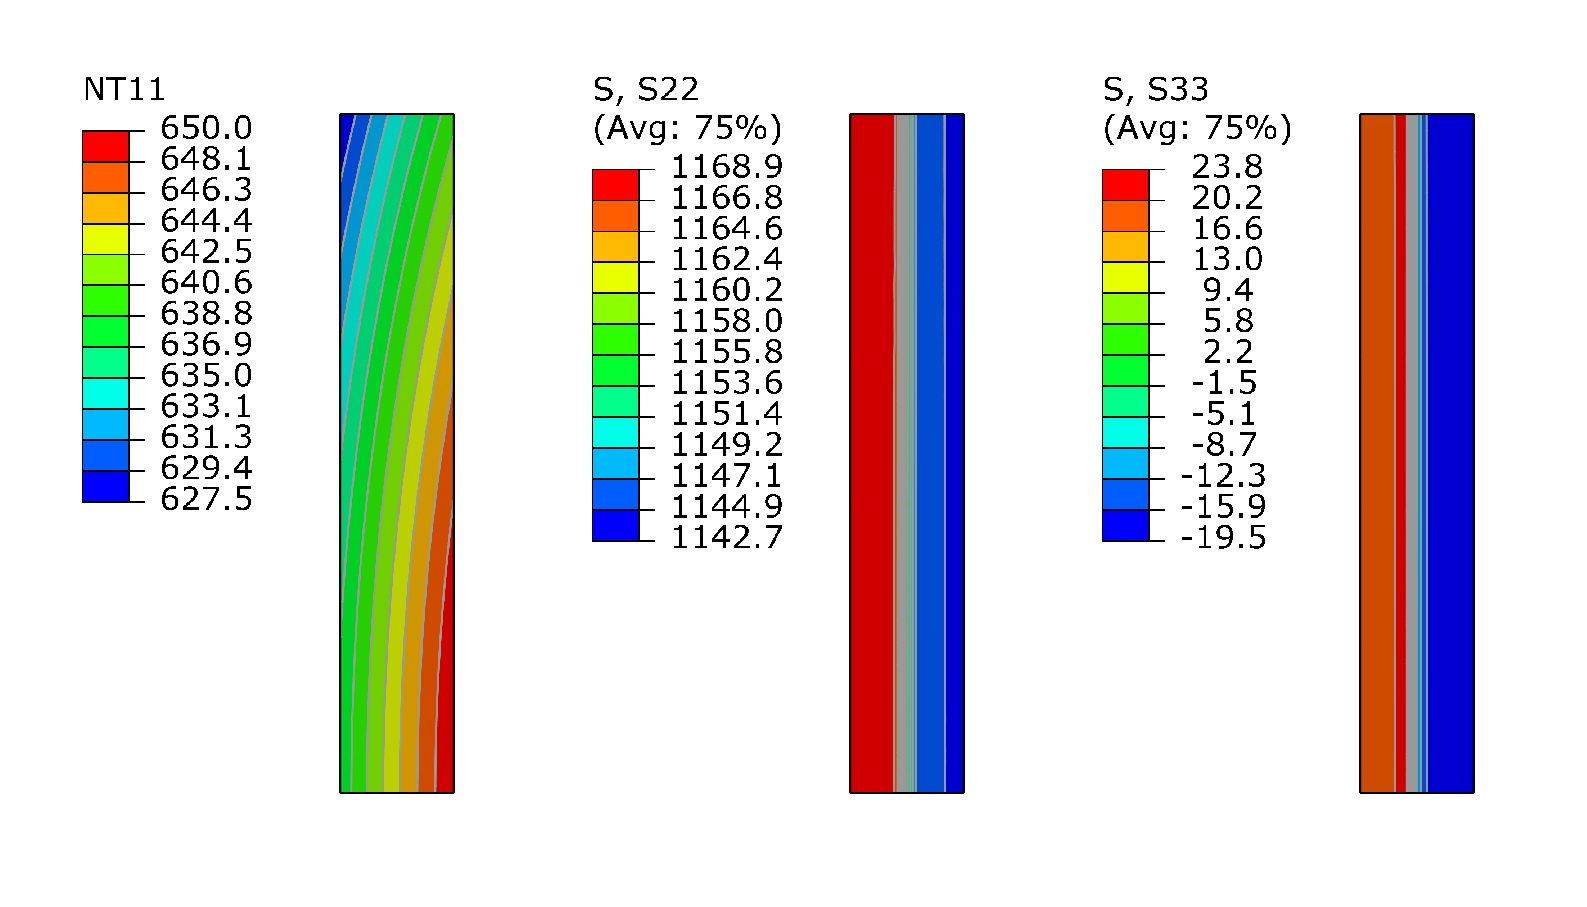
\includegraphics[width=14cm]{FEM_result.jpg}}
  \caption{Diagram of simulated axial temperature gradients and the resulting, thermally induced axial stress components at maximum temprature (650$^{\circ}$C) during the TGMF-IP test with the mechanical strain amplitude of 0.8\% (NT11: temperature in ℃, S22: axial stress in MPa, S33: hoop stress in MPa).}
  \label{Fig:FEM_result}
\end{figure*}

\begin{figure}[htbp]
  \centering
    \begin{overpic}[width=8cm]{plot_temperature_along_gauge_length.pdf}
      \put(75,65){\fcolorbox{white}{white}{(a)}}
    \end{overpic}
    \begin{overpic}[width=8cm]{plot_temperature_along_radial_direction.pdf}
      \put(75,65){\fcolorbox{white}{white}{(b)}}
    \end{overpic}
  \caption{Diagram of the simulated temperature and stress components at the maximum temprature (650$^\circ$C) during the TGMF-IP test with the mechanical strain amplitude of 0.8\%, (a) axial direction (b) radial direction.}
  \label{Fig:plot_temperature_stress}
\end{figure}

Under TGMF-IP loading condition, the mechanical load and temperature simultaneously reach their respective maximum or minimum values. \autoref{Fig:FEM_result} shows the computational results of TGMF-IP test with the mechanical strain amplitude of 0.8\%. The maximum temperature occurs at the point B in \autoref{Fig:FE_model}.
\autoref{Fig:plot_temperature_stress}(a) shows the temperature and axial stress distribution of the internal and external surface along the axial direction when the temperature reached its maximum value during the TGMF-IP cycle.
The abscissa axis is the distance from the center section of the test specimen ($y$-axis in \autoref{Fig:FE_model}). The temperature gradients induce an axial stress deviation of ca. 25 MPa between the inner and outer surface of the specimen.
The temperature and axial stress distribution of the internal and external surface along the radial direction are displayed in \autoref{Fig:plot_temperature_stress}(b), when the temperature reached its maximum value during the TGMF-IP cycle.
The abscissa axis is the distance from the center axis to the outer surface of the test specimen ($r$-axis in \autoref{Fig:FE_model}).
The temperature gradients induce a radial stress deviation of ca. 50 MPa between the inner and outer surface of the specimen.




\section{Fractography}
% 通过裂纹扩展区域的形貌和疲劳辉纹的方向我们可以推测出裂纹萌生的位置,如图\autoref{Fig:crack_initiation}所示,图中箭头所示为裂纹萌生的位置。我们可以观测到显著的稳态裂纹扩展和裂纹失稳扩展区域,对于650$^{\circ}$C等温疲劳(IF)试验,试样断口比TMF和TGMF断口更加平整,疲劳扩展区面积较大。
% 对于所有的等温疲劳(IF)和热机械疲劳(TMF)试验,疲劳裂纹都萌生于试样表面或近表面的缺陷处以及优先氧化区域并以沿枝晶和穿晶混合的方式在晶粒内部扩展。
% 虽然温度梯度导致了TGMF试样外表面附加了一定程度的压应力,但对于本文中的试验参数,所有的热梯度机械疲劳(TGMF)试验,疲劳裂纹都萌生于试样外表面。

We can infer the location of the crack initiation by the fractography of the crack propagation area and the direction of the fatigue striation.
Typical fractographs in the region of crack initiation are shown in \autoref{Fig:crack_initiation_TGMF}, and the arrows show the locations of the crack initiation. For both TGMF-IP and TGMF-OP loadings, crack initiation, and subsequent failure have been identified as being initiated at the outer surface of the specimen.

\autoref{Fig:fatigue_striations_TGMF} shows the fractography of stable crack propagation. For the TGMF tests, the SEM investigations reveal that the dominant failure mechanism is changing with the phase angle of the thermal loading and mechanical loading, $\theta_{T-\varepsilon}$.
In \autoref{Fig:fatigue_striations_TGMF}(a) and (b), the fracture surfaces under TGMF-IP loading displays evident grain boundaries and slight fatigue striations. Consequently, it can be concluded that a mixture of transgranular and intergranular fracture mode is present in the TGMF-IP test, and the intergranular fracture plays a dominant role.
Well-developed fatigue striations are observed in \autoref{Fig:fatigue_striations_TGMF}(c) and (d), which reveal transgranular crack growth is predominant during out-of-phase thermomechanical tests.

\begin{figure}[ht]
  \centering
    \begin{overpic}[width=8.0cm]{7206-1.jpg}
      \put(0,65){\fcolorbox{white}{white}{(a)}}
      \put(70,40){\color{white}\thicklines\vector(3,-1){20}}
    \end{overpic}
    \begin{overpic}[width=8.0cm]{7207-1.jpg}
      \put(0,65){\fcolorbox{white}{white}{(b)}}
      \put(60,40){\color{white}\thicklines\vector(1,-1){13}}
    \end{overpic}
  \caption{Locations of crack initiation from the TGMF tests: (a) TGMF-IP 0.65\%, (b) TGMF-OP 0.65\%. Arrows denote the crack initiation locations.}
  \label{Fig:crack_initiation_TGMF}
\end{figure}

% 对五种不同试验条件下疲劳断口的扩展区和瞬间断裂区进行观察,如图\autoref{Fig:fatigue_striations}所示,图中箭头为裂纹扩展方向。结果表明,TMF-OP和TGMF-OP的疲劳辉纹最为清晰(图\autoref{Fig:fatigue_striations}(c,e,f)),650$^{\circ}$C IF,TMF-IP和TGMF-IP并未看到明显的疲劳辉纹(图\autoref{Fig:fatigue_striations}(a),(b),(d)),这是由于在650$^{\circ}$C IF,TMF-IP和TGMF-IP试验条件下裂纹张开扩展时处于较高温度,断口表面经受了较多
% 高温氧化损伤的原因。
% 而三种载荷条件下的瞬间失稳断裂区则非常相似,与拉伸试样的断口形貌相似。

\begin{figure*}[htbp]
  \centering{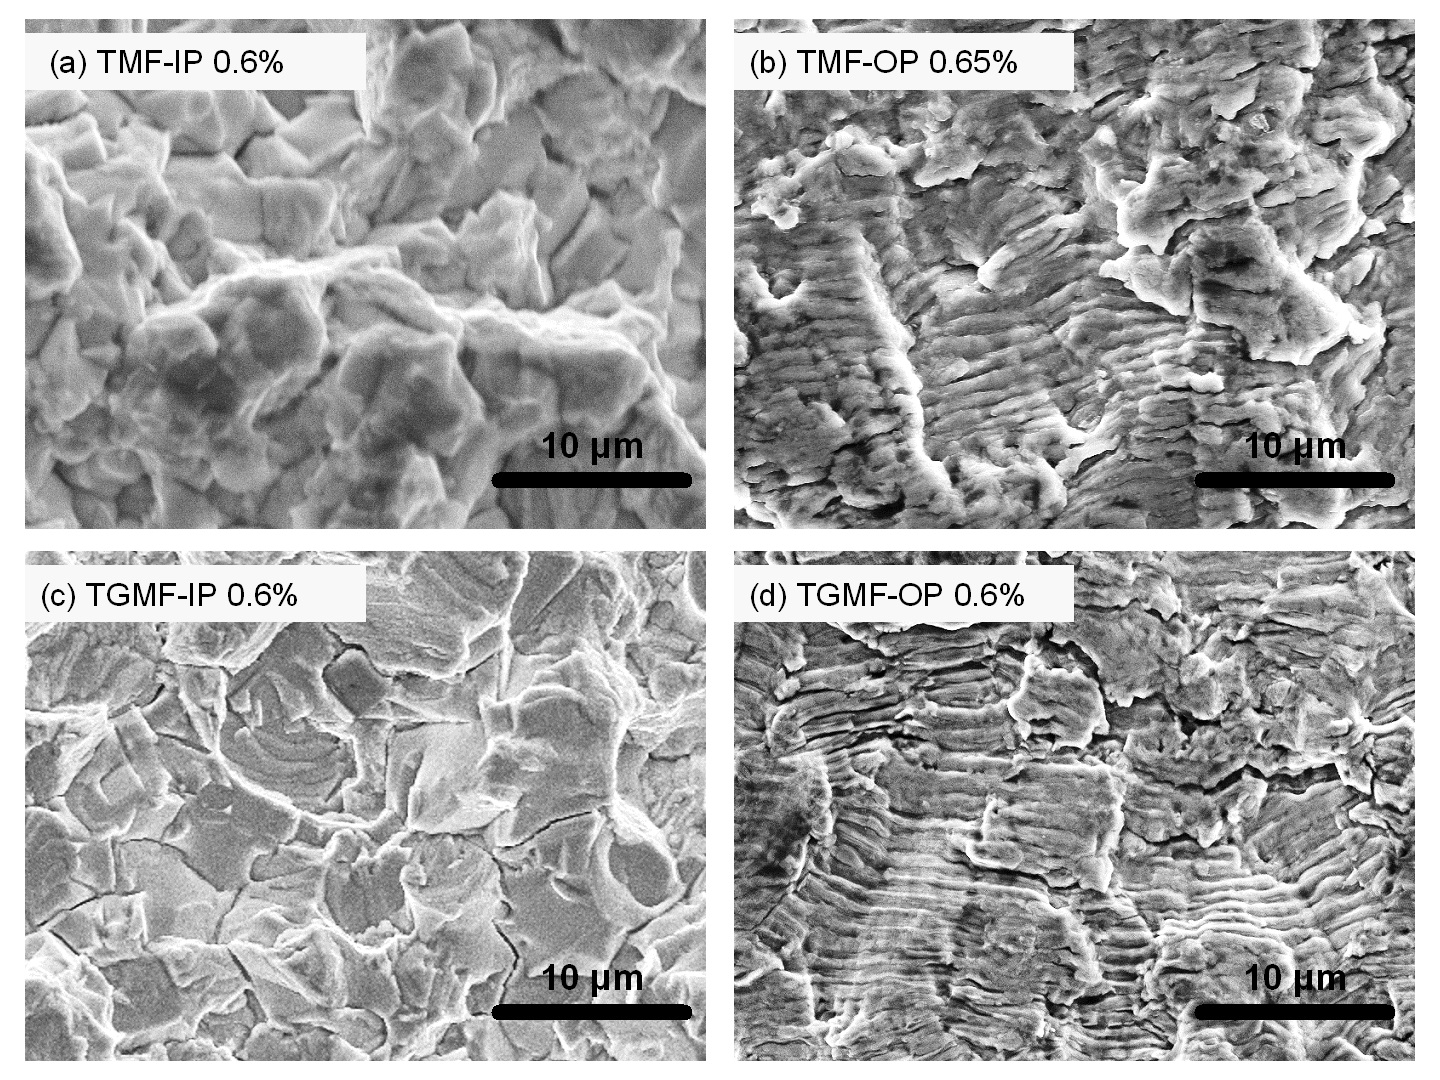
\includegraphics[width=16cm]{Fractography.jpg}}
  \caption{Fractographs of fracture surfaces from the area of stable crack propagation.}
  \label{Fig:fatigue_striations_TGMF}
\end{figure*}

\newpage
\section{Fatigue life assessment of TGMF}

In the present section, several known fatigue models are selected to evaluate the fatigue life of the nickel-based superalloy under both TMF and TMGF loading conditions. Combined with the critical plane concept the models are well developed and verified for isothermal fatigue.

\subsection{Brown-Miller Model}
Based on the critical plane concepts \cite{Brown2006}, Wang and Brown \cite{Wang1993} proposed that the Kandil, Brown and Miller fatigue model \cite{Kandil1982} can be reformulated in the form of the equivalent shear strain amplitude, as
\begin{equation}
\frac{{\Delta \hat \gamma }}{2} = \frac{{\Delta {\gamma _{\max}}}}{2} + S\Delta {\varepsilon _{\rm n}},
\label{Equ:ShearStrainBM}
\end{equation}
where ${{\Delta \hat \gamma }}/{2}$ is the equivalent shear strain range \cite{Wang1993}. $\Delta {\varepsilon _{\rm n}}$ represents the normal strain acting on the plane with the maximum shear strain range $\Delta {\gamma _{\max}}$. The material dependent parameter $S$ represents the influence of the normal strain on the crack propagation.

\subsection{Fatemi-Socie Model}
Fatemi and Socie \cite{Fatemi1988} proposed that the normal strain term in Eq. (\ref{Equ:ShearStrainBM}) should be replaced by the normal stress.
The equivalent shear strain amplitude is defined as
\begin{equation}
\frac{{\Delta \hat \gamma }}{2} = \frac{{\Delta {\gamma _{\max }}}}{2}\left( {1 + k\frac{{{\sigma _{\rm n,\max}}}}{{{\sigma _{\rm y}}}}} \right),
\end{equation}
where
$\sigma _{\rm n,\max}$ is the maximum normal stress on the critical plane suffering from the maximum shear strain range $\Delta {\gamma _{\max}}$, and $k$ is a material parameter. The sensitivity of the material to the normal stress is reflected in the ratio $k/\sigma _{\rm y}$.

\subsection{Smith-Watson-Topper Model}
The SWT model \cite{smith1970stress} can be extended to multiaxial fatigue assessment based on the principal strain range and the maximum stress on the plane of the principal strain range, that is,
\[
{\sigma _{\rm n, \max}}\frac{{\Delta \varepsilon }}{2} = \frac{{{{\sigma '}_{\rm f}}^2}}{E}{\left( {2{N_{\rm f}}} \right)^{2b}} + {\sigma '_{\rm f}}{\varepsilon '_{\rm f}}{\left( {2{N_{\rm f}}} \right)^{b + c}}.
\]

\subsection{Chu-Conle-Bonnen Model}
An additional energy-based fatigue model suggested by Chu et al. \cite{Chu1993} is expressed as
\begin{eqnarray}
{\left( {{\tau _{\rm n}}\frac{{\Delta \gamma }}{2} + {\sigma _{\rm n }}\frac{{\Delta \varepsilon }}{2}} \right)_{\max }} &=& 1.02\frac{{{{\sigma '}_{\rm f}}^2}}{E}{\left( {2{N_{\rm f}}} \right)^{2b}} \\
&& + 1.04{{\sigma '}_{\rm f}}{{\varepsilon '}_{\rm f}}{\left( {2{N_{\rm f}}} \right)^{b + c}}.
\end{eqnarray}
Note the difference in the strain energy in comparing with the Liu's models. The critical plane should provide the maximum strain energy in the whole loading range and in all directions.

\subsection{Liu's Virtual Strain Energy Models}
The virtual tensile strain energy based model suggested by Liu \cite{Liu1993} can be written as
\begin{eqnarray}
{\left( {\Delta {\sigma _{\rm n}}\Delta {\varepsilon _{\rm n}}} \right)_{\max }} + \left( {\Delta \tau \Delta \gamma } \right) &=& \frac{{4{{\sigma '}_{\rm f}}^2}}{E}{\left( {2{N_{\rm f}}} \right)^{2b}}
\\
& & + 4{{\sigma '}_{\rm f}}{{\varepsilon '}_{\rm f}}{\left( {2{N_{\rm f}}} \right)^{b + c}}.
\end{eqnarray}
Above the critical plane is defined from maximizing the virtual tensile strain energy ${\Delta {\sigma _{\rm n}}\Delta {\varepsilon _{\rm n}}}$, termed as Liu I model. 

\subsection{TMF Model}
Based on the Liu's virtual tension strain energy model, Sun \cite{SUN2019228} introduced a fatigue model for the multi-axial TMF life prediction, which given by,
\begin{equation}
\begin{aligned}
\left[ {A{{\left( {\Delta {\sigma _{\rm n}}\Delta {\varepsilon _{\rm n}}} \right)}_{\max }} + B\left( {\Delta \tau \Delta \gamma } \right)} \right]\left( {\frac{2}{{1 - {R_\sigma }}}} \right)\\
= \frac{{4{{\sigma '}_{\rm f}}^2}}{E}{\left( {2{N_{\rm f}}} \right)^{2b}} + 4{{\sigma '}_{\rm f}}{{\varepsilon '}_{\rm f}}{\left( {2{N_{\rm f}}} \right)^{b + c}},
\end{aligned}
\label{Equ:TMF_model}
\end{equation}
where $A$ is defined as
\begin{equation}
A = {\left[ {1 + C\int_{{t_0}}^{{t_0} + {t_{cyc}}} {\eta \left( t \right)\exp \left( {\frac{{ - Q\left( t \right)}}{{RT\left( t \right)}}} \right){\rm{d}}t} } \right]^k},
\label{Equ:A}
\end{equation}
in which $\eta \left( t \right)$ is stress triaxiality, $R$ is the ideal gas constant ($8.31\times10^{-3}$ kJ/mol$\cdot$K), the time integral is from the start time $t_0$ of the cycle to the end time $t_0 + t_{cyc}$, $t_{cyc}$ is the period of the tests, $C$ and $k$ are material constants.
In Eq. (\ref{Equ:A}), $Q$ presents \cite{Warren2006,Warren2008}
\begin{equation}
Q\left( t \right) = {Q_0} - \upsilon _0^*{\sigma _{\rm n}}\left( t \right)\left( {1 - \frac{{{\sigma _{\rm n}}\left( t \right)}}{{2{\sigma _{\rm ult}}}}} \right),
\label{Equ:creep_activation_energy}
\end{equation}
where $Q_0$ is the the intrinsic activation energy, $\upsilon _0^*$ represents the intrinsic activation volume, $\sigma_{\rm ult}$ is the ultimate stress at the maximum temperature and $\sigma_{\rm n}(t)$ is the normal stress of the critical plane.
As given in \cite{Warren2008}, the activation energy $Q_0$ is set to 240 kJ/mol and the intrinsic activation volume $\upsilon _0^*$ is $3.51\times10^{-4}$ $\rm{m}^{3}/\rm{mol}$. The ultimate strength $\sigma_{\rm ult}$ of Inconel 718 at 650$^\circ$C was measured as $1305$ MPa in monotonic tensile tests. The coefficients $k$, $B$ and $C$ are determined from minimizing the life prediction mean square error. Finally, $k$ equals 1.2, $B$ is 0.49, and $C$ is set to $1.29\times10^{12}$ s$^{-1}$.

\subsection{Fatigue life prediction based on the conventional fatigue models}
The Brown-Miller's model, Fatemi-Socie's model, Smith-Watson-Topper's model, Chu-Conle-Bonnen's model, Liu's Energy model and TMF model (Equation \eqref{Equ:TMF_model}) are tried to evaluate the thermal gradient mechanical fatigue.
\autoref{Fig:life_prediction_TGMF} shows the comparison between predicted and experimental fatigue life of the IF, TMF-IP, TMF-OP, TGMF-IP and TGMF-OP tests. It is observed that the predicted fatigue lives of all models are too much non-conservative for the thermal gradient mechanical fatigue tests.
\begin{figure*}
   \centering
   \begin{overpic}[width=7.0cm]{NF-NP-TGMF-BM.pdf}
     \put(65,20){\fcolorbox{white}{white}{(a) BM}}
   \end{overpic}
   \begin{overpic}[width=7.0cm]{NF-NP-TGMF-FS.pdf}
     \put(70,20){\fcolorbox{white}{white}{(b) FS}}
   \end{overpic}

   \begin{overpic}[width=7.0cm]{NF-NP-TGMF-SWT.pdf}
     \put(70,20){\fcolorbox{white}{white}{(c) SWT}}
   \end{overpic}
   \begin{overpic}[width=7.0cm]{NF-NP-TGMF-Chu.pdf}
     \put(70,20){\fcolorbox{white}{white}{(d) CCB}}
   \end{overpic}

   \begin{overpic}[width=7.0cm]{NF-NP-TGMF-Liu1.pdf}
     \put(70,20){\fcolorbox{white}{white}{(e) Liu I}}
   \end{overpic}
   \begin{overpic}[width=7.0cm]{NF-NP-TGMF-Study.pdf}
     \put(70,20){\fcolorbox{white}{white}{(f) TMF}}
   \end{overpic}
  \caption{Comparison between predicted fatigue life and experimental results of multiaxial thermomechanical fatigue tests. (a) Brown-Miller model; (b) Fatemi-Socie model; (c) Smith-Watson-Topper model; (d) Chu-Conle-Bonnen model; (e) Liu Tension Energy model; (f) TMF model (Equation \eqref{Equ:TMF_model}).}
  \label{Fig:life_prediction_TGMF}
\end{figure*}

It can be observed that the TMF model has the best agreement in the prediction of the TMF and TGMF tests.
% 图\autoref{Fig:plot_exp_fatigue_life_TMF_TGMF}分别比较了TMF和TGMF在同相位和反相位时的疲劳寿命。
% 可以发现,同相位和反相位的情况下TGMF寿命都要低于TMF寿命,由于两组试验的温度循环相同,唯一不同的是试件径向方向的温度梯度,因此可以认为温度梯度对材料寿命有不利的影响,同时比较图\autoref{Fig:plot_exp_fatigue_life_TMF_TGMF}(a)和(b),在同相位的情况下,温度梯度导致的寿命减少比反向位试验更加明显。
% 根据上一节的分析可知,Chu能量模型在TMF-IP,TMF-OP和TGMF-OP的预测上有比较好的结果,表\autoref{Tab:FatigueCoefficient}列举出了Chu模型计算过程中的参数,其中$\phi$为临界面与中心截面的夹角,$\sigma_{n,max}$为该临界面上在循环过程中的最大正应力,$T$,$\partial T/\partial y$和$\partial T/\partial r$为最大正应力处所对应的温度与温度梯度。
% 在Chu能量模型的基础上,增加温度梯度的修正项,新的寿命模型如下:
Therefore, based on the TMF model, a correction term of the temperature gradient is multiplied on the right-hand side of Equation \eqref{Equ:TMF_model}. The fatigue life model for TGMF is suggested as:
\begin{equation}
\begin{aligned}
f\left( {T,\nabla T} \right)\left[ {A{{\left( {\Delta {\sigma _{\rm n}}\Delta {\varepsilon _{\rm n}}} \right)}_{\max }} + B\left( {\Delta \tau \Delta \gamma } \right)} \right]\left( {\frac{2}{{1 - {R_\sigma }}}} \right) \\ 
= \frac{{4{{\sigma '}_f}^2}}{E}{\left( {2{N_f}} \right)^{2b}} + 4{{\sigma '}_f}{{\varepsilon '}_f}{\left( {2{N_f}} \right)^{b + c}}.
\end{aligned}
\label{Equ:TGMF_model}
\end{equation}
The correction term of the temperature gradient is defined as:
\begin{equation}
f\left( {T,\nabla T} \right) = \left( {1 + g\frac{{\left\| {\nabla T} \right\|}}{{{T_{{\rm{melt}}}} - {T_{{\sigma _{\rm n,\max }}}}}}} \right),
\label{Equ:TGMF_term}
\end{equation}
where ${T_{{\rm{melt}}}}$ is the melting point of the material, and ${T_{{\sigma _{\rm n,\max }}}}$ is the temperature corresponding to the maximum normal stress, $g$ is a model parameter in the unit of mm. For the Nickel-based superalloy Inconel 718, we set ${T_{{\rm{melt}}}}=1300$ $^\circ$C. The model parameter $g$ is determined by the optimization algorithm to minimize the life prediction
mean-squared error, and $g$ is determined as 3.47 mm in the present work. ${\left\| {\nabla T} \right\|}$ is the temperature gradient and given by:
\begin{equation}
\left\| {\nabla T} \right\| = \sqrt {{{\left( {\frac{{\partial T}}{{\partial x}}} \right)}^2} + {{\left( {\frac{{\partial T}}{{\partial y}}} \right)}^2} + {{\left( {\frac{{\partial T}}{{\partial z}}} \right)}^2}}.
\end{equation}
Considering Equation \eqref{Equ:TGMF_model} and \eqref{Equ:TGMF_term}, when $\left\| {\nabla T} \right\|=0$, $f\left( {T,\nabla T} \right)=1$, then Equation \eqref{Equ:TGMF_model} reduce to Equation \eqref{Equ:TMF_model}.

\autoref{Tab:Temperature_gradient} lists the parameters in the calculation of the proposed TGMF model, where $\varphi$ is the angle of the critical plane, $T_{\sigma_{\rm n,\max}}$ is the maximum normal stress during the cycle on the critical plane, $T_{\sigma_{\rm n,\max}}$, $\partial T/\partial y$ and $\partial T/\partial r$ are the temperature and temperature gradients corresponding to the maximum normal stress location.
\autoref{Fig:TGMF_model} shows the fatigue life assessment of the TGMF tests. As shown in \autoref{Fig:TGMF_model}(a), the fatigue damage parameters vs. experimental fatigue lives is illustrated. The fatigue damage parameters show good correlation with experimental fatigue lives of TGMF-IP and TGMF-OP tests. In \autoref{Fig:TGMF_model}(b), one can observe that based on the proposed model (Equation \eqref{Equ:TGMF_model}), most of the predicted fatigue lives are within the scatter band with a factor of 2. It shows a good agreement with the experimental and predicted fatigue lives.

\autoref{Fig:plot_fatigue_life_quantitative_evaluation_tgmf} shows a quantitative assessment of TGMF life prediction results. As introduced in chapter 6, two statistical parameters ${T_{\rm N}}$ (Equation \eqref{Equ:TN}) and ${T_{\rm RMS}}$ (Equation \eqref{Equ:TRMS}) are used to evaluate the conformity of the predicted and experimental TGMF lives. The results in \autoref{Fig:plot_fatigue_life_quantitative_evaluation_tgmf} illustrate that the present TGMF model generates the best mean value in comparing with all other models, while the present TGMF model possesses the least scattering. Combining the two parameters, the present model provides the best result in predicting the fatigue life for all experiments.

\begin{table*}[htbp]
  \centering
  \caption{Stress, strain, temperature and temperature gradient on the material plane.}
    \begin{tabular}{lcccccccrr}
    \toprule
    Load Type & $\Delta\varepsilon/2$ & $\varphi$ & $\Delta\sigma$ & $\Delta\varepsilon$ & $T_{\sigma_{\rm n,\max}}$   & $\partial T/\partial y$ & $\partial T/\partial r$ & $N_{\rm{f}}$ & $N_{\rm{p}}$ \\
          & [\%]  & [$^{\circ}$] & [MPa] & [\%]  & [$^\circ$C]   & [$^\circ$C/mm] & [$^\circ$C/mm] & [cycle] & [cycle] \\
    \midrule
    TGMF-IP & 0.425   & 0     & 1058.4  & 0.85  & 650   & -11.6  & 0.092  & 1066  & 552 \\
      & 0.50   & 0     & 1298.3  & 0.99  & 650   & -11.6  & 0.092  & 208   & 126 \\
      & 0.60   & 0     & 1827.8  & 1.29  & 650   & -11.6  & 0.092  & 107   & 102 \\
      & 0.70   & 0     & 1758.6  & 1.28  & 650   & -11.6  & 0.092  & 50    & 78 \\
      & 0.80   & 0     & 1917.3  & 1.87  & 650   & -11.6  & 0.092  & 48    & 39 \\
    \midrule
    TGMF-OP & 0.425   & 0     & 1562.6  & 0.78  & 300   & -6.5  & 0.044  & 3387  & 11784 \\
      & 0.50   & 0     & 1680.5  & 1.02  & 300   & -6.5  & 0.044  & 864   & 1637 \\
      & 0.60   & 0     & 1834.4  & 1.42  & 300   & -6.5  & 0.044  & 375   & 697 \\
      & 0.80   & 0     & 1981.1  & 2.00  & 300   & -6.5  & 0.044  & 128   & 26 \\
    \bottomrule
    \end{tabular}%
  \label{Tab:Temperature_gradient}%
\end{table*}%

\begin{figure}[htbp]
  \centering
  \begin{overpic}[width=8cm]{F-NF-TGMF-Study2.pdf}
    \put(86,15){{(a)}}
  \end{overpic}
  \begin{overpic}[width=8cm]{NF-NP-TGMF-Study2.pdf}
    \put(86,18){{(b)}}
  \end{overpic}
  \caption{Computational results of the TGMF tests, based on the present model: (a) Fatigue damage parameter versus experimental fatigue lifetime, (b) Comparison of the predicted fatigue lifetime and experimental fatigue lifetime.}
  \label{Fig:TGMF_model}
\end{figure}

\autoref{Fig:plot_fatigue_life_quantitative_evaluation_tgmf} shows a quantitative assessment of fatigue life prediction results. According to the Refs. \cite{KAROLCZUK201439,WALAT201473,SKIBICKI201718}, two statistical parameters are used to evaluate the conformity of the predicted $N_{\rm p}$ and experimental $N_{\rm f}$ fatigue lives. The mean scatter of fatigue life,
\begin{equation}
{T_{\rm N}} = {10^{\bar E}}
\label{Equ:TN}
\end{equation}
with
\begin{equation}
\bar E = \frac{1}{n}\sum\limits_{i = 1}^n {\log \left( {\frac{{{N_{{\rm f},i}}}}{{{N_{{\rm p},i}}}}} \right)},
\end{equation}
illustrates the comparison of the mean value of experimental and predicted lives. Above $n$ is the total number of the compared results, and the subscript $i$ indicates the $i$th. result. $T_{\rm N} = 1$ shows the mean value of experimental and predicted lives are identical. $T_{\rm N} > 1$ means the predicted fatigue lives are conservative, and $T_{\rm N} < 1$ means the predicted fatigue lives are non-conservative. The statistical parameter $T_{\rm N}$ does not provide any information on the dispersion of fatigue life.

The other parameter is the root mean square error of the fatigue life,
\begin{equation}
{T_{\rm RMS}} = {10^{{E_{\rm RMS}}}},
\label{Equ:TRMS}
\end{equation}
with
\begin{equation}
{E_{\rm RMS}} = \sqrt {\frac{1}{n-1}\sum\limits_{i = 1}^n {\left[{{\log }}\left( {\frac{{{N_{{\rm f},i}}}}{{{N_{{\rm p},i}}}}} \right) \right]^2}}.
\end{equation}
The root mean square error is applied to measure the differences between fatigue lives obtained from predictions and the results from experiments. $T_{\rm RMS} = 1$ represents the mean value and the statistical dispersion of experimental and predicted lives are equal. In other cases, $T_{\rm RMS}$ is larger than 1, and the larger value of $T_{\rm RMS}$ represents the more dispersion between the experimental and predicted lives.

The results in \autoref{Fig:plot_fatigue_life_quantitative_evaluation_tgmf} illustrate that the present model generates the best mean value in comparing with all other models, while the present model possesses the least scattering. Combining the two parameters, the present model provides the best result in predicting the fatigue life for all experiments.

\begin{figure}[htbp]
  \centering
  \begin{overpic}[width=8.0cm]{plot_fatigue_life_quantitative_evaluation_tgmf_TN.png}
  \put(84,65){\fcolorbox{white}{white}{(a)}}
  \end{overpic}
  \begin{overpic}[width=8.0cm]{plot_fatigue_life_quantitative_evaluation_tgmf_TRMS.png}
  \put(84,65){\fcolorbox{white}{white}{(b)}}
  \end{overpic}
  \caption{The quantitative evaluation of the TGMF life prediction results: (a) $T_{\rm{N}}$, (b) $T_{\rm{RMS}}$.}
  \label{Fig:plot_fatigue_life_quantitative_evaluation_tgmf}
\end{figure}

\section*{Acknowledgement:}

\bibliographystyle{unsrt}            % bibliography style
% \bibliographystyle{plain}            % bibliography style
% \bibliography{bibliography}          % personal bibliography file
\bibliography{mybib}                 % personal bibliography file

\end{document} 